%% ----------------------------------------------------------------
%% Thesis.tex -- MAIN FILE (the one that you compile with LaTeX)
%% ---------------------------------------------------------------- 

% Set up the document
\documentclass[a4paper, 12pt, oneside]{Thesis}  % Use the "Thesis" style, based on the ECS Thesis style by Steve Gunn
\graphicspath{{Figures/}}  % Location of the graphics files (set up for graphics to be in PDF format)

% Include any extra LaTeX packages required
\usepackage[square, numbers, comma, sort&compress]{natbib}  % Use the "Natbib" style for the references in the Bibliography
\usepackage{verbatim}  % Needed for the "comment" environment to make LaTeX comments
\usepackage{vector}  % Allows "\bvec{}" and "\buvec{}" for "blackboard" style bold vectors in maths
\usepackage[romanian]{babel}
\usepackage{epsfig}
\usepackage{listings}
\hypersetup{urlcolor=blue, colorlinks=true}  % Colours hyperlinks in blue, but this can be distracting if there are many links.

\lstset{
	language=[Visual]C++,
	keywordstyle=\bfseries\ttfamily\color[rgb]{0,0,1},
	identifierstyle=\ttfamily,
	commentstyle=\color[rgb]{0.133,0.545,0.133},
	stringstyle=\ttfamily\color[rgb]{0.627,0.126,0.941},
	showstringspaces=false,
	basicstyle=\small,
	numberstyle=\footnotesize,
	numbers=left,
	stepnumber=1,
	numbersep=10pt,
	tabsize=2,
	breaklines=true,
	prebreak = \raisebox{0ex}[0ex][0ex]{\ensuremath{\hookleftarrow}},
	breakatwhitespace=false,
	aboveskip={1.5\baselineskip},
  columns=fixed,
  upquote=true,
  extendedchars=true,
% frame=single,
% backgroundcolor=\color{lbcolor},
}

%% ----------------------------------------------------------------
\begin{document}
\frontmatter	  % Begin Roman style (i, ii, iii, iv...) page numbering

% Set up the Title Page
\title  {Interfa\c{t}a SCPI de comand\u{a} pentru un generator de semnal}
\authors  {\texorpdfstring
            {\href{your web site or email address}{ing. Cristian Paraschiv}}
            {Cristian Paraschiv}
            }
\addresses  {\groupname\\\deptname\\\univname}  % Do not change this here, instead these must be set in the "Thesis.cls" file, please look through it instead
\date       {Septembrie 2012}
\subject    {}
\keywords   {}

\maketitle
%% ----------------------------------------------------------------

\setstretch{1.5}  % It is better to have smaller font and larger line spacing than the other way round

% Define the page headers using the FancyHdr package and set up for one-sided printing
\fancyhead{}  % Clears all page headers and footers
\rhead{\thepage}  % Sets the right side header to show the page number
\lhead{}  % Clears the left side page header

\pagestyle{fancy}  % Finally, use the "fancy" page style to implement the FancyHdr headers

%% ----------------------------------------------------------------
% Declaration Page required for the Thesis, your institution may give you a different text to place here
%\Declaration{
%
%\addtocontents{toc}{\vspace{1em}}  % Add a gap in the Contents, for aesthetics
% }
\clearpage  % Declaration ended, now start a new page

%% ----------------------------------------------------------------
% The "Funny Quote Page"
\pagestyle{empty}  % No headers or footers for the following pages

\null\vfill
% Now comes the "Funny Quote", written in italics
%\textit{``Write a funny quote here.''}

%\begin{flushright}
%If the quote is taken from someone, their name goes here
%\end{flushright}

\vfill\vfill\vfill\vfill\vfill\vfill\null
\clearpage  % Funny Quote page ended, start a new page
%% ----------------------------------------------------------------

% The Abstract Page
\addtotoc{Abstract}  % Add the "Abstract" page entry to the Contents
\abstract{
\addtocontents{toc}{\vspace{1em}}  % Add a gap in the Contents, for aesthetics


}

\clearpage  % Abstract ended, start a new page
%% ----------------------------------------------------------------

\setstretch{1.3}  % Reset the line-spacing to 1.3 for body text (if it has changed)

% The Acknowledgements page, for thanking everyone
%\acknowledgements{
%\addtocontents{toc}{\vspace{1em}}  % Add a gap in the Contents, for aesthetics

%The acknowledgements and the people to thank go here, don't forget to include your project advisor\ldots

%}

\clearpage  % End of the Acknowledgements
%% ----------------------------------------------------------------

\pagestyle{fancy}  %The page style headers have been "empty" all this time, now use the "fancy" headers as defined before to bring them back


%% ----------------------------------------------------------------
\lhead{\emph{Cuprins}}  % Set the left side page header to "Contents"
\tableofcontents  % Write out the Table of Contents

%% ----------------------------------------------------------------
\lhead{\emph{Lista de figuri}}  % Set the left side page header to "List if Figures"
\listoffigures  % Write out the List of Figures

%% ----------------------------------------------------------------
\lhead{\emph{Lista de tabele}}  % Set the left side page header to "List of Tables"
\listoftables  % Write out the List of Tables

%% ----------------------------------------------------------------
\setstretch{1.5}  % Set the line spacing to 1.5, this makes the following tables easier to read

%% ----------------------------------------------------------------

%% ----------------------------------------------------------------
%% ----------------------------------------------------------------
% End of the pre-able, contents and lists of things
% Begin the Dedication page

\setstretch{1.5}  % Return the line spacing back to 1.3

\pagestyle{empty}  % Page style needs to be empty for this page
%\dedicatory{For/Dedicated to/To my\ldots}

\addtocontents{toc}{\vspace{2em}}  % Add a gap in the Contents, for aesthetics


%% ----------------------------------------------------------------
\mainmatter	  % Begin normal, numeric (1,2,3...) page numbering
\pagestyle{fancy}  % Return the page headers back to the "fancy" style

% Include the chapters of the thesis, as separate files
% Just uncomment the lines as you write the chapters

% Chapter 1

\chapter{Introducere} % Write in your own chapter title
\label{Capitolul1}
\lhead{Capitolul 1. \emph{Introducere}} % Write in your own chapter title to set the page header

\section{Motiva\c{t}ie}

Dezvoltarea \c{s}i utilizarea sistemelor de m\u{a}surare programabile au fost explorate pe scar\u{a} larg\u{a}. Posibilitatea de a modifica procedura de m\u{a}surare prin simpla schimbare a algoritmului executat de un calculator f\u{a}r\u{a} a \^{i}nlocui componentele hardware face activitatea experimental\u{a} mai u\c{s}oara.

Timp de mul\c{t}i ani, instrumentele electronice au fost u\c{s}or de identificat. De\c{s}i variaz\u{a} \^{i}n m\u{a}rime \c{s}i func\c{t}ionalitate, toate sunt sub forma unei cutii, av\^{a}nd un panou frontal \c{s}i un display. Acestea sunt foarte puternice \c{s}i sunt concepute pentru a executa una sau mai multe sarcini men\c{t}ionate de c\u{a}tre v\^{a}nz\u{a}tor.

Cu toate acestea, utilizatorul nu le poate extinde sau particulariza. Butoanele, circuitele interne \c{s}i func\c{t}iile disponibile utilizatorului sunt speficice naturii instrumentului. Adoptarea pe scar\u{a} larg\u{a} a PC-ului \^{i}n ultimii dou\u{a}zeci de ani a dat na\c{s}tere unui nou mod de m\u{a}surare \c{s}i automatizare pentru ingineri.

Un prim model conceptual al instrumenta\c{t}iei bazat\u{a} pe calculator este prezentat \^{i}n figura de mai jos:

\begin{figure}[tbp]
  \centering
  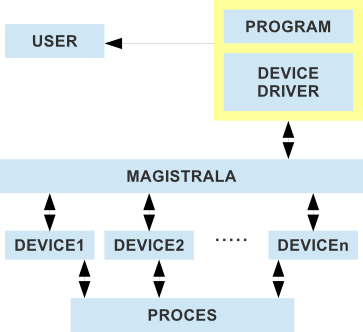
\epsfig{file=Figuri/model_instrumentatie.eps,width=0.5\linewidth,clip=}
  \caption{Model al instrumenta\c{t}iei bazate pe calculator}
  \label{figsistem}
\end{figure}

Un singur utilizator controleaz\u{a} sistemul. Exist\u{a} o singur\u{a} structur\u{a} de control, format\u{a} din utilizator \c{s}i programul care comand\u{a} instrumentele ata\c{s}ate magistralei.

Instrumentele sistemului pot folosi fie o comunica\c{t}ie serial\u{a}, bazat\u{a} pe standardul RS-232, fie o comunica\c{t}ie paralela, bazat\u{a} pe standardul GPIB.

Scopul \emph{Standard Commands for Programmable Instruments (SCPI)} este acela de a facilita reducerea timpului de dezvoltare pentru programele implementate \^{i}n sistemele de m\u{a}surare \c{s}i control precum \c{s}i de a permite schimbarea aparatelor (eventual produse de firme diferite) \^{i}n cadrul aceluia\c{s}i sistem de m\u{a}surare condus de calculator. Acest lucru se realizeaz\u{a} prin introducerea unor comenzi standardizate c\u{a}tre aparate \c{s}i a unor tipuri posibile de r\u{a}spuns al acestora. Spre exemplu, comanda:
\begin{center}
	\begin{verbatim}
	MEASURE:FREQ?
	\end{verbatim}
\end{center}

are aceea\c{s}i sintax\u{a} pentru toate aparatele de un anumit tip (de exemplu, multimetre) fabricate de diver\c{s}i producatori - consisten\c{t}\u{a} vertical\u{a} - dar \c{s}i pentru aparate cu func\c{t}ii diferite (de exemplu, osciloscoape, num\u{a}r\u{a}toare) - consisten\c{t}\u{a} orizontal\u{a}.

SCPI nu este un limbaj de programare (cum sunt, de exemplu, Pascal sau C), ci un limbaj de comenzi care define\c{s}te comenzile c\u{a}tre aparate, parametrii \c{s}i formatul acestora. SCPI furnizeaz\u{a} un \c{s}ir de caractere ASCII care vor fi transmise prin rutine specifice aparatelor unde vor fi, apoi, prelucrate prin intermediul limbajului TMSL (\emph{Hewlett-Packard's Test and Measurement System Language}).

SCPI s-a dezvoltat, \^{i}n principal, p\u{a}str\^{a}nd o compatibilitate cu norma IEEE-488 \c{s}i utiliz\^{a}nd formatul de date al acestei norme. Cu toate acestea, utilizarea SCPI nu este limitat\u{a} la interfa\c{t}a IEEE-488, comenzile acestuia put\^{a}nd fi transmise \c{s}i prin interfe\c{t}ele VXI sau RS-232 \c{s}i, \^{i}n plus, fiind continuu supus complet\u{a}rilor necesitate de dezvoltarea hardware-ului specific, \^{i}n urma recomand\u{a}rilor f\u{a}cute de un consor\c{t}iu de firme, alc\u{a}tuit din reprezentan\c{t}i ai leader-ilor pe pia\c{t}a instrumentelor de m\u{a}surare: Hewlett-Packard, Tektronix, Fluke (Philips), Keithley, Rohde\&Schwarz etc.

Cu toate c\u{a} SCPI define\c{s}te comenzile specifice aparatelor de m\u{a}surare "inteligente", nu sunt indicate nici un fel de date tehnice privind exactitatea, rezolu\c{t}ia, domeniul de m\u{a}surare ale acestora; astfel nu poate fi \^{i}n totalitate garantat\u{a} compatibilitatea aparatelor \^{i}n cadrul unui sistem comandat prin intermediul SCPI.

\section{Scop}

Aceast\u{a} lucrare \^{i}\c{s}i propune analizarea \c{s}i implementarea unei interfe\c{t}e SCPI de comand\u{a} pentru generatorul de semnal BK 4070. Din cauza faptului c\u{a} acest generator suport\u{a} un anumit set de comenzi \c{s}i comunica\c{t}ie serial\u{a}, prin standardul RS-232, s-a dorit integrarea acestuia \^{i}ntr-un sistem mai mare, compatibil cu standardul SCPI.

Se vor folosi aplica\c{t}iile Lex \c{s}i Yacc pentru generarea gramaticii \c{s}i sintaxei interfe\c{t}ei SCPI, urm\^{a}nd ca aplica\c{t}ia generat\u{a} s\u{a} trimit\u{a} serial comenzi c\u{a}tre generatorul de semnal.

\section{Rezumat}

Lucrarea este structurat\u{a} \^{i}n trei par\c{t}i. Prima parte \^{i}\c{s}i propune descrierea aspectelor teoretice ale standardului SCPI. Se vor prezenta structura comenzilor precum \c{s}i clasele \^{i}n care se incadreaz\u{a} acestea.

A doua parte \^{i}\c{s}i propune prezentarea utilitarelor Lex \c{s}i Yacc. Vor fi descrise regulile pentru scrierea fi\c{s}ierelor, modul de execu\c{t}ie pentru generarea unui translator.

\^{I}n final, a treia parte \c{s}i cea mai important\u{a}, prezint\u{a} implementarea \c{s}i func\c{t}ionarea interfe\c{t}ei SCPI de comand\u{a} pentru un generator de semnal.
 % Introduction
% Chapter 1

\chapter{SCPI (Standard Commands for Programmable Instruments)
} % Write in your own chapter title
\label{Capitolul2}
\lhead{Capitolul 2. \emph{SCPI (Standard Commands for Programmable Instruments)}} % Write in your own chapter title to set the page header

Domeniul instrumenta\c{t}iei a folosit dintotdeauna tehnologie electronic\u{a} larg utilizat\u{a}. Principiul acului de ceas a fost folosit la scar\u{a} larg\u{a} pentru construirea de instrumente de m\u{a}surat analogice. Capacitorul variabil, rezistorul variabil au fost utilizate primele \^{i}n dezvoltarea instrumenta\c{t}iei electronice. Apoi tehnologia display-ului a fost \^{i}mprumutat\u{a} din televiziune \^{i}n vederea utiliz\u{a}rii pentru aparatele de analizat \c{s}i cele osciloscop.

Astazi, sistemele viabile de calcul desktop \c{s}i notebook constituie, printre altele suportul pentru noua genera\c{t}ie de instrumente - instrumentele virtuale. Acestea sunt proiectate \c{s}i realizate de utilizator conform cu nevoile specifice.

\^{I}n 1965, Hewlett-Packard dezvolta HPIB (Hewlett Packard Interface Bus) \^{i}n vederea conectarii instrumentelor programabile la sistemele de calcul. Datorit\u{a} ratei mari de transfer, nominal 1 Mbytes/s, aceast\u{a} interfa\c{t}\u{a} a c\^{a}\c{s}tigat imediat popularitate. Ulterior s-a impus ca standardul numit IEEE 488, apoi evolu\^{a}nd la IEEE 488.1. Ast\u{a}zi se utilizeaz\u{a} mai larg denumirea de GPIB (General Purpose Interface Bus) \^{i}n locul celei de HPIB. 

Standard Commands for Programable Instruments a luat structura de comenzi definit\u{a} \^{i}n cadrul IEEE 488.2 \c{s}i a creat un mediu de programare unic, transparent. SCPI, fiind independent de partea hardware, poate fi implementat peste alte tipuri de standarde, cum ar fi RS-232 sau GPIB. Mai concret, SCPI \emph{define\c{s}te un set standard de comenzi pentru controlul dispozitivelor de testare \c{s}i m\u{a}surare \^{i}n sistemele de instrumente}.

Un sistem de instrumente reprezint\u{a} un grup de dispozitive de testare \c{s}i m\u{a}surare, conectate printr-o magistral\u{a} de comunica\c{t}ie la un calculator de control, apelat de controlerul de sistem. Un sistem de instrumente poate include dispozitive de sine-st\u{a}t\u{a}toare, cum ar fi instrumente de tip IEEE 488, sau placi-instrumente, \^{i}nglobate \^{i}ntr-un sistem.

Controlerul de sistem trimite comenzi unuia sau mai multor instrumente prin intermediul magistralei. Aceste comenzi sunt numite mesaje de program. Instrumentele trimit \^{i}napoi r\u{a}spunsuri c\u{a}tre magistral\u{a}. Mesajul r\u{a}spuns poate fi rezultatul unei m\u{a}sur\u{a}tori, o setare a instrumentului sau un mesaj de eroare. C\^{a}nd un mesaj de program genereaza direct un raspuns, acesta se nume\c{s}te interogare. SCPI reprezint\u{a} un limbaj uniform \c{s}i consistent pentru controlul instrumentelor de testare \c{s}i m\u{a}surare.

\section{Scopul SCPI}
Principalul scop al SCPI este s\u{a} reduc\u{a} generarea sistematica a programelor pentru echipamente automate de testare (Automatic Test Equipment - ATE). Instrumentele SCPI sunt foarte flexibile, accept\^{a}nd un domeniu larg de formate de comenzi \c{s}i parametri.

Cheia unei astfel de program\u{a}ri consistente const\u{a} \^{i}n reducerea diferitelor modalit\u{a}\c{t}i de a controla func\c{t}iile instrumentelor. Filosofia SCPI este ca acelea\c{s}i func\c{t}ii ale unui instrument s\u{a} fie controlate de acelea\c{s}i comenzi SCPI.

SCPI este proiectat \^{i}n vederea adaug\u{a}rii de noi comenzi \^{i}n orice perioad\u{a} de timp, f\u{a}r\u{a} ca acestea s\u{a} cauzeze probleme de programare a instrumentelor. Pe m\u{a}sura ce apar noi instrumente, exist\u{a} inten\c{t}ia de a men\c{t}ine compatibilitatea programului de control cu alte instrumente SCPI deja existente.

Avantajul folosirii SCPI pentru programatorul sistemului ATE este reducerea timpului de \^{i}nv\u{a}\c{t}are de a programa noi instrumente SCPI, chiar dup\u{a} programarea unui alt instrument tot de tip SCPI.

Furniz\^{a}nd un mediu consistent de programare, \^{i}nlocuirea unui instrument SCPI cu alt echipament SCPI \^{i}ntr-un sistem ATE va necesita de obicei mai pu\c{t}in efort dec\^{a}t cu instrumente non-SCPI.

Toate instrumentele SCPI trebuie s\u{a} fie \^{i}n conformitate cu specifica\c{t}iile IEEE 488.2 \c{s}i vor pune \^{i}n aplicare toate comenzile comune declarate obligatorii:

\begin{table}[h]
	\begin{center}
	\begin{tabular}{|l|l|}
		\hline
		Mnemonica & Nume\\
		\hline
		*CLS & Clear Status Command\\
		*ESE & Standard Event Status Enable Command\\
		*ESE? & Standard Event Status Enable Query\\
		*ESR? & Standard Event Status Register Query\\
		*IDN? & Identification Query\\
		*OPC & Operation Complete Command\\
		*OPC? & Operation Complete Query\\
		*RST & Reset Command\\
		*SRE & Service Request Enable Command\\
		*SRE? & Service Request Enable Query\\
		*STB? & Read Status Byte Query\\
		*TST? & Self Test Query\\
		*WAI & Wait-to-Continue Command\\
		\hline
	\end{tabular}
	\end{center}
	\caption{Lista de comenzi obligatorii}
\end{table}

\begin{figure}[!htb]
	\centering
	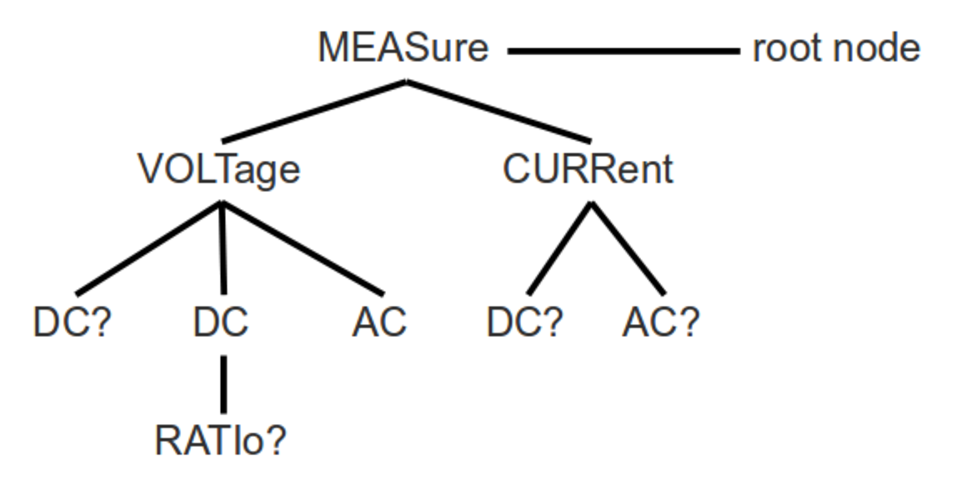
\includegraphics[scale=0.8]{./Figuri/structuracomanda.eps}
	\caption{Structura unei comenzi SCPI}
	\label{structuracomanda}
\end{figure}

\section{Comenzi suprapuse \c{s}i secven\c{t}iale}
IEEE 488.2 define\c{s}te o deosebire \^{i}ntre comenzile suprapuse \c{s}i cele secven\c{t}iale. A\c{s}a cum este definit\u{a} \^{i}n standard, o comand\u{a} secven\c{t}ial\u{a} este una care \^{i}\c{s}i termin\u{a} executarea \^{i}nainte de pornirea comenzii urm\u{a}toare. O comand\u{a} suprapus\u{a} este una care nu termin\u{a} executarea \^{i}nainte de \^{i}nceperea comenzii urm\u{a}toare.

IEEE 488.2 define\c{s}te trei comenzi comune, *OPC, *WAI, *OPC?, pe care un dispozitiv conduc\u{a}tor \^{i}l poate folosi pentru a-\c{s}i sincroniza func\c{t}ionarea la executarea de comenzi suprapuse.

Fiecare comand\u{a} suprapus\u{a} a fost asociat\u{a} cu un Pending Operation Flag. Dispozitivul configureaz\u{a} acest steag la valoarea \emph{true} atunci c\^{a}nd trece de la comanda corespunz\u{a}toare din blocul Execution Control c\u{a}tre blocul Device Action. Dispozitivul configureaz\u{a} steagul pe valoarea \emph{false} c\^{a}nd func\c{t}ionarea dispozitivului este terminat\u{a} sau este intrerupt\u{a}.

\section{Comenzi optionale}
Exist\u{a} comenzi facultative, depinz\^{a}nd de posibilita\c{t}ile instrumentului. C\^{a}nd un dispozitiv nu suport\u{a} to\c{t}i parametrii alternativi care sunt permi\c{s}i pentru o comand\u{a} SCPI, el poate s\u{a} pun\u{a} \^{i}n aplicare o subselec\c{t}ie a acestor valori, numai cu excep\c{t}ia \^{i}n care au fost altfel declarate. De exemplu, dac\u{a} un instrument pune \^{i}n aplicare numai func\c{t}iile RECTangular \c{s}i UNIform pentru comenzile CALCulate:TRANSform:WINDow, se poate genera o eroare de la oricara alt parametru declarat (Flattop, Hamming, etc). Oricum, un dispozitiv trebuie s\u{a} pun\u{a} \^{i}n aplicare to\c{t}i parametrii unei comenzi SCPI multi-parametru.

Un instrument cu un monitor care este configurat s\u{a} fie \^{i}n permanen\c{t}\u{a} pornit nu are nevoie de punerea \^{i}n aplicare a unei comenzi pentru pornire/oprire. Dac\u{a} un instrument are o configura\c{t}ie fix\u{a}, \^{i}n care o setare nu corespunde cu valoarea *RST, atunci instrumentul va pune \^{i}n aplicare comanda pentru acea setare.

\subsection{Interpretarea tabelei de comenzi}
Tabelele de comenzi sunt folosite ca s\u{a} defineasc\u{a} un set de comenzi SCPI. Un tabel prezint\u{a} comenzile, rela\c{t}iile lor ierarhice, parametrii \^{i}nrudi\c{t}i (\^{i}n cazul \^{i}n care exist\u{a}), \c{s}i nota\c{t}ii sau comentarii asociate acestora. Tabelul este format din trei coloane: una pentru cuv\^{a}ntul cheie (Keyword), una pentru forma parametrului (Parameter Form) \c{s}i una pentru nota\c{t}ii sau comentarii (Notes).

Coloana cuv\^{a}ntului cheie (Keyword) furnizeaz\u{a} numele comenzii. Numele comenzii reale const\u{a} din unul sau mai multe cuvinte cheie, comenzile SCPI baz\^{a}ndu-se pe o structur\u{a} ierarhic\u{a}, cunoscut\u{a} de asemenea ca structur\u{a} arborescent\u{a}. \^{I}ntr-n astfel de sistem, comenzile asociate sunt grupate \^{i}mpreun\u{a} sub un nod comun \^{i}n ierarhie. Acestea \c{s}i ramurile asem\u{a}n\u{a}toare sunt conectate \^{i}ntr-un num\u{a}r mai mare sau mai mic, p\^{a}n\u{a} ce \^{i}nt\^{a}lnesc r\u{a}d\u{a}cina structurii arborescente. Cu c\^{a}t un nod este mai aproape de r\u{a}d\u{a}cin\u{a}, cu at\^{a}t este considerat mai important \^{i}n ierarhie. Pentru a ob\c{t}ine o ramur\u{a} special\u{a} sau o comand\u{a} special\u{a}, trebuie s\u{a} fie specificat\u{a} calea unde se afl\u{a}. Aceast\u{a} cale este reprezentat\u{a} \^{i}n tabele prin plasarea celui mai superior nod \^{i}n ierarhie, \^{i}n pozi\c{t}ia cea mai din st\^{a}nga. Nodurile inferioare \^{i}n ierarhie sunt mutate cu o pozi\c{t}ie \^{i}nspre partea dreapt\u{a}, dedesuptul nodului-parinte.

Parantezele drepte sunt utilizate pentru cuvintele cheie op\c{t}ionale atunci c\^{a}nd se programeaza comanda; instrumentul va trebui s\u{a} proceseze aceast\u{a} comand\u{a} ca av\^{a}nd acela\c{s}i efect, indiferent dac\u{a} nodul-op\c{t}iune este omis de programator. Un astfel de nod este denumit nod implicit (default node).

Majusculele din cadrul cuv\^{a}ntului cheie al unei comenzi indic\u{a} forma prescurtat\u{a} care este la fel de valabila ca \c{s}i forma complet\u{a}.

Coloana cu forma parametrului indic\u{a} numarul \c{s}i ordinea parametrului \^{i}ntr-o comand\u{a}, precum \c{s}i valorile sale. O comand\u{a} poate permite folosirea unui tip de parametru SCPI, literal, sau o combina\c{t}ie a celor dou\u{a}.
 
\^{I}n coloana cu forma parametrului, o serie de caractere au o semnifica\c{t}ie special\u{a}. Ca \c{s}i mai sus, parantezele drepte sunt folosite pentru a indica unul sau mai mul\c{t}i parametri care sunt op\c{t}ionali atunci c\^{a}nd se controleaz\u{a} instrumentul. Acoladele sunt folosite pentru indicarea parametrilor care sunt folosi\c{t}i de mai multe ori sau deloc. Bara vertical\c{a} poate fi interpretat\u{a} ca "sau" \c{s}i este folosit\u{a} pentru a separa diferite op\c{t}iuni ale parametrilor alternativi. 

Coloana nota\c{t}ii: forma interog\u{a}rii unei comanzi este generat\u{a} adaug\^{a}nd un semn de \^{i}ntrebare la ultimul cuv\^{a}nt cheie. Oricum, nu toate comenzile au o forma specific\u{a} a interog\u{a}rii, \c{s}i alte comenzi exist\u{a} numai sub forma de interogare.

Exemplu:
\begin{table}[h]
	\begin{center}
	\begin{tabular}{|l|l|l|}
		\hline
		KEYWORD & PARAMETER FORM & NOTES\\
		\hline
		:FREQuency &  & \\
		\verb [:CW] & \textless numeric value\textgreater & \\
		\ \ \ \ :AUTO & \textless Boolean\textgreater & \\
		:CENTer & \textless numeric value\textgreater & \\
		:SPAN & \textless numeric value\textgreater & \\
		\hline		
	\end{tabular}
	\end{center}
\end{table}

Pentru setarea valoarii frecven\c{t}ei pentru un semnal sinusoidal continuu (contnuous wave - CW), comanda ar trebui s\u{a} aiba urm\u{a}toarea forma: 
\begin{center}
FREQuency:CW 2000000
\end{center}
Deoarece nodul [:CW] este op\c{t}ional, se poate utiliza urm\u{a}toarea form\u{a} de comand\u{a}: 
\begin{center}
FREQuency: 2000000
\end{center}
Pentru setarea valorii AUTO, poate fi utilizat\u{a} una din urm\u{a}toarele forme, depinz\^{a}nd, ca \c{s}i mai sus, de nodul CW care este op\c{t}ional:
\begin{center}
FREQuency:CW:AUTO OFF

FREQuency:AUTO OFF
\end{center}
Forma interog\u{a}rii a comenzii AUTO este una din cele de mai jos: 
\begin{center}
FREQuency:CW:AUTO?

FREQuency:AUTO?
\end{center}

\section{Construirea structurii arborescente}
Comenzile SCPI sunt bazate pe o structur\u{a} ierarhic\u{a}. Aceasta permite ca acela\c{s}i cuv\^{a}nt cheie s\u{a} fie \^{i}ntrebuin\c{t}at \^{i}n repetate r\^{a}nduri pentru scopuri diferite, f\u{a}c\^{a}nd ca mnemonicele s\u{a} aibe o pozi\c{t}ie unic\u{a} \^{i}n ierarhie. Aceasta se realizeaz\u{a} \^{i}n vederea evit\u{a}rii suprapunerii cu oricare alta abreviere aflat\u{a} la acela\c{s}i nivel. Folosind comenzile ierarhice ar trebui s\u{a} se elimine nevoia de mnemonice cu mai multe cuvinte.

\section{Sintaxa mesajelor program}
Un mesaj program const\u{a} din una sau mai multe comenzi SCPI trimise de la controler la instrument pentru a comanda o ac\c{t}iune sau pentru a interoga instrumentul. \^{I}n figura \ref{fig1} este reprezentat schematic un mesaj program.

\begin{figure}[htp]
 \centering
 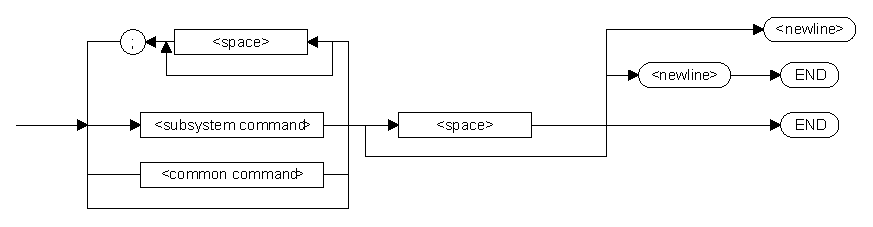
\includegraphics[scale=0.7]{Figuri/fig1_scpi_meas.eps}
 \caption{Sintaxa mesajului program}
 \label{fig1}
\end{figure}

Simbolul punct \c{s}i virgul\u{a} este folosit pentru separarea comenzilor din acela\c{s}i grup. De exemplu se poate trimite urm\u{a}torul mesaj pentru a seta starea portului de ie\c{s}ire digital (8 linii de ie\c{s}ire) \c{s}i pentru a citi starea portului:

\begin{center}
\begin{verbatim}
:OUTPut:255; :OUTPut?
\end{verbatim}
\end{center}

Unirea unor comenzi din grupuri diferite se realizeaz\u{a} folosind punct \c{s}i virgul\u{a} \c{s}i dou\u{a} puncte. De exemplu citirea registrului Operation Status \c{s}i setarea portului digital de ie\c{s}ire:

\begin{center}
\begin{verbatim}
:STATus:OPERation:CONDition? ;:OUTPut:255
\end{verbatim}
\end{center}

Pentru terminarea unui mesaj program se pot folosi urm\u{a}toarele terminatoare:
\begin{itemize}
	\item \textless  newline\textgreater sau caracterul \textless  NL\textgreater
	\item \textless  END\textgreater care este interpretat ca \c{s}i \textless  NL\textgreater
	\item \textless  newline\textgreater\textless  END \textgreater
\end{itemize}

Terminarea mesajului program reseteaz\u{a} calea comenzii SCPI curente la nivel radacin\u{a}.

Urm\u{a}toarele sec\c{t}iuni descriu sintaxa comenzilor SCPI generale \c{s}i comenzilor SCPI subsistem.

\subsection{Sintaxa comenzilor SCPI generale}
Figura \ref{fig2} descrie sintaxa comenzilor SCPI generale.

\begin{figure}[htp]
 \centering
 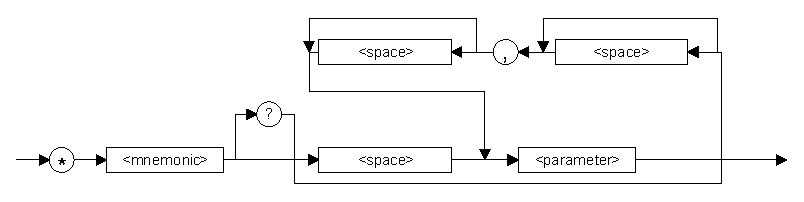
\includegraphics[scale=0.8]{Figuri/fig2_scpi_meas.eps}
 \caption{Sintaxa comenzilor generale}
 \label{fig2}
\end{figure}

Comenzile SCPI generale \^{i}ncep cu simbolul asterix (*). Comenzile sunt de tip case-insensitive. De exemplu urm\u{a}toarele comenzi produc acela\c{s}i rezultat:
\begin{verbatim}
*RST
*rst
*Rst
\end{verbatim}

Interog\u{a}rile necesit\u{a} simbolul \emph{semn de \^{i}ntrebare} la sf\^{a}r\c{s}itul comenzii:
\begin{verbatim}
*IDN?
\end{verbatim}

\subsection{Sintaxa comenzilor SCPI subsistem}
Figura \ref{fig3} descrie sintaxa comenzilor SCPI subsistem.

\begin{figure}[htp]
 \centering
 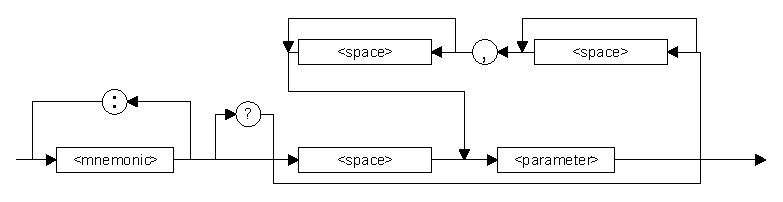
\includegraphics[scale=0.8]{Figuri/fig3_scpi_meas.eps}
 \caption{Sintaxa comenzilor SCPI subsistem}
 \label{fig3}
\end{figure}

Se folose\c{s}te simbolul \emph{dou\u{a} puncte} pentru separarea cuvintelor cheie:
\begin{verbatim}
:STATus:OPERation:ENABle
\end{verbatim}

Interog\u{a}rile necesit\u{a} simbolul semn de \^{i}ntrebare la sf\^{a}r\c{s}itul comenzii:
\begin{verbatim}
:STATus:OPERation:CONDition?
\end{verbatim}

\section{Sintaxa mesajelor r\u{a}spuns}
Un mesaj r\u{a}spuns const\u{a} din date \^{i}ntr-un format specific SCPI care au fost cerute instrumentului de c\u{a}tre controler.

Figura \ref{fig4} descrie sintaxa mesajului r\u{a}spuns al unui instrument:

\begin{figure}[htp]
 \centering
 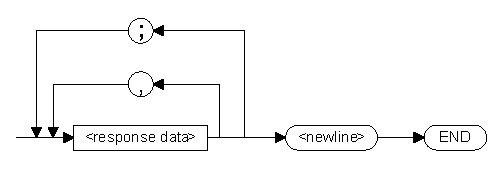
\includegraphics[scale=1]{Figuri/fig4_scpi_meas.eps}
 \caption{Sintaxa mesajului r\u{a}spuns}
 \label{fig4}
\end{figure}

Mesajele r\u{a}spuns pot con\c{t}ine at\^{a}t virgula c\^{a}t \c{s}i punct \c{s}i virgula ca \c{s}i separatori. C\^{a}nd o singur\u{a} comand\u{a} de interogare returneaz\u{a} valori multiple, se folose\c{s}te virgula pentru a separa fiecare element. C\^{a}nd sunt trimise mai multe interog\u{a}ri \^{i}ntr-un singur mesaj, grupurile de date corespunz\u{a}toare fiec\u{a}rei interog\u{a}ri sunt separate prin punct \c{s}i virgul\u{a}.

Terminatorul mesajului r\u{a}spuns este \^{i}ntotdeauna \textless  newline\textgreater\textless \^END\textgreater.

\section{Antete de program}
Antetele de program sunt cuvintele cheii care identific\u{a} comanda. Instrumentele vor accepta \c{s}i varianta cu comenzi cu majuscule \c{s}i cea cu litere mici, instrumentele nef\u{a}c\^{a}nd distinc\c{t}ie \^{i}ntre acestea.

Antetele de program se compun din dou\u{a} tipuri distincte \c{s}i anume antetele de comand\u{a} \c{s}i antetele de control ale instrumentului.

\begin{figure}[htp]
 \centering
 
\includegraphics[scale=1]{Figuri/scpi_ro_1.eps}
 \caption{Sintaxa antetelor de comanda}
 \label{fig6}
\end{figure}

\begin{figure}[htp]
 \centering
 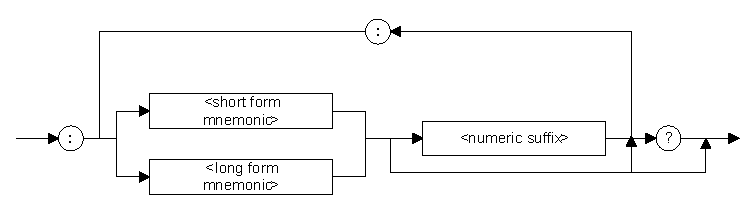
\includegraphics[scale=1]{Figuri/scpi_ro_2.eps}
 \caption{Sintaxa antetelor de control}
 \label{fig6}
\end{figure}

\section{Interog\u{a}rile}
Toate comenzile, numai \^{i}n cazul c\^{a}nd sunt altfel notate, au \^{i}n plus \c{s}i o form\u{a} de interogare. A\c{s}a cum este definit \^{i}n IEEE 488. 2, o interogare este un antet de comand\u{a} cu un simbol al unui semn de \^{i}ntrebare ad\u{a}ugat (de exemplu FREQ: CENT?). C\^{a}nd un formular de \^{i}ntrebare al unei comenzi este primit, setarea curent\u{a} asociat\u{a} comenzii este plasat\u{a} \^{i}n buffer-ul de ie\c{s}ire. R\u{a}spunsurile interog\u{a}rii nu includ antetul de comand\u{a}. Executare unui formular de \^{i}ntrebare nu are efectele secundare. O excep\c{t}ie este \^{i}n subsistemul MEASurement, unde set\u{a}rile instrumentului ar putea s\u{a} schimbe rezultatul m\u{a}sur\u{a}torii.

Atat formularul de comand\u{a} c\^{a}t \c{s}i cel de interogare trebuie s\u{a} fie implementate, excep\c{t}ie f\u{a}c\^{a}ndu-se \^{i}n cazul \^{i}n care un comentariu care indic\u{a} altceva apare \^{i}n sumarul cuvintelor ceie. Chiar \c{s}i c\^{a}nd o comand\u{a} accept\u{a} numai o singur\u{a} selec\c{t}ie, at\^{a}t formularul de comand\u{a} c\^{a}t \c{s}i cel de interogare vor trebui s\u{a} fie aplicate.

C\^{a}nd informa\c{t}iile de caracter se \^{i}ntrebuin\c{t}eaz\u{a} pentru un parametru, ambele variante, longform \c{s}i shortform, vor trebui s\u{a} fie recunoscute. Dac\u{a} comanda are un formular de \^{i}ntrebare cu informa\c{t}ii de r\u{a}spuns de caracter, valoarea shortform este \^{i}ntotdeauna \^{i}ntoars\u{a}.

C\^{a}nd parametrii numerici sunt interoga\c{t}i, rezultatul se va \^{i}ntoarce \^{i}n unit\u{a}\c{t}ile de m\u{a}sur\u{a} de baz\u{a}, \^{i}n cazul \^{i}n care nu se specific\u{a} sau impune altfel. C\^{a}nd unele din diferitele unit\u{a}\c{t}i pot fi considerate fundamentale (de exemplu: dBuV, dBm), atunci unit\u{a}\c{t}ile rezultatului vor trebui s\u{a} fie detaliate \^{i}n descrierea r\u{a}spunsului interog\u{a}rii.

\section{Parametrii}
 SCPI folose\c{s}te formele de parametri descrise \^{i}n standardul IEEE 488.2, cu cateva restric\c{t}ii adi\c{t}ionale. Trebuie observat c\u{a} SCPI specific\u{a} valorile pentru toate comenzile prin *RST. \^{I}n unele cazuri, aceste valori resetate sunt dependente de dispozitiv, dar parametrii de m\u{a}surare trebuie s\u{a} fie regla\c{t}i fa\c{t}\u{a} de o valoare determinist\u{a} pentru acel instrument special, care la r\^{a}ndul s\u{a}u trebuie s\u{a} fie documentat\u{a} \^{i}n manualul instrumentului.

\subsection{Date de program de tip caracter}
Unde exist\u{a} posibilitatea, acelea\c{s}i reguli de trunchiere se \^{i}ntrebuin\c{t}eaz\u{a} at\^{a}t pentru parametri c\^{a}t \c{s}i pentru antete. Oricum, \^{i}n multe cazuri standardele industriale r\u{a}m\^{a}n \^{i}n urm\u{a}. De exemplu, IDC este o alegere mai bun\u{a} pentru curent continuu dec\^{a}t vreo regul\u{a} definit\u{a} \^{i}n cadrul SCPI, pur \c{s}i simplu deoarece el este un standard cu acceptare larg\u{a}. \^{I}n plus, c\^{a}teva informa\c{t}ii de program tip caracter sunt definite anticipat, precum extensiile de genul date de program tip num\u{a}r zecimal (\textless  DECIMAL NUMERIC PROGRAM DATA\textgreater).

\subsection{Date de program tip num\u{a}r zecimal}
Elemente numerice se vor \^{i}ntrebuin\c{t}a numai pentru reprezentarea cantit\u{a}\c{t}ilor numerice. Ele nu se vor \^{i}ntrebuin\c{t}a pentru selectare de func\c{t}ii la un comutator de pozi\c{t}ie. Implement\u{a}rile vor accepta informa\c{t}iile numerice a\c{s}a cum sunt descrise \^{i}n IEEE 488.2. Cu toate acestea, orice num\u{a}r care depa\c{s}e\c{s}te + -9. 9E37 va genera o eroare de execu\c{t}ie (-222 date necuprinse \^{i}n domeniu). Numerele vor fi rotunjite c\^{a}t mai aproape de valoarea corect\u{a} pe care acel instrument o accept\u{a} f\u{a}r\u{a} eroare.

\subsection{Definirea valorii numerice}
Elementul numeric zecimal este prescurtat \^{i}n felul urm\u{a}tor: \textless  numeric\_value\textgreater . Anumite forme de date de program de tip caracter, \textless CHARACTER PROGRAM DATA\textgreater , sunt definite precum formularele speciale de numere. Acestea sunt: MINimum, MAXimum, DEFault, UP, DOWN, Not a Number(NAN), Infinity \c{s}i Negative Infinity( NINF):

\begin{itemize}
	\item DEFault - Parametrul special \textless numeric\_value\textgreater DEFault poate fi furnizat astfel \^{i}nc\^{a}t s\u{a} permit\u{a} instrumentului s\u{a} selecteze o valoare pentru un parametru. C\^{a}nd DEFault este expediat, instrumentul va selecta o valoare care este crezut\u{a} s\u{a} fie c\^{a}t mai \^{i}n conformitate cu dorin\c{t}a clientului. Setarea poate s\u{a} fie dependent\u{a} de dispozitiv sau poate s\u{a} fie definit\u{a} precum o parte a aceastui standard. Folosirea de DEFault este facultativ\u{a} \^{i}n cadrul unei structuri comand\u{a}-cu-comand\u{a}. Comenzi individuale vor avea rolul de a indica unde este necesar DEFault.
	\item MINimum/MAXimum - Ace\c{s}ti parametri speciali de tip numeric vor fi furni-za\c{t}i pentru specificarea valorilor de limit\u{a} pentru parametru. MINimum/MAXimum vor trebui s\u{a} fie interogabili prin trimiterea urm\u{a}toarei linii de program: \textless header\textgreater? MAXimum|MINimum. Valoarea Maximum se refer\u{a} la valoarea cea mai mare pe care acea func\c{t}ie poate \^{i}n mod curent s\u{a} fie expediat\u{a}, iar Minimum se refer\u{a} la valoarea cea mai mic\u{a} la care func\c{t}ia poate fi reglat\u{a}.
	\item UP/DOWN - Un instrument are posibilitatea de a permite folosirea de pa\c{s}i pentru unele sau toate intr\u{a}rile numerice. Dac\u{a} sunt utiliza\c{t}i pa\c{s}i, cuvintele cheie UP \c{s}i DOWN se vor \^{i}ntrebuin\c{t}a ca \c{s}i parametri numerici care s\u{a} execute pa\c{s}ii. Pa\c{s}ii mai pot s\u{a} fie ajustabili prin nodul pasului pentru fiecare parametru individual. Instrumentul poate s\u{a} \^{i}nainteze cu un pas atunci c\^{a}nd  UP sau DOWN este primit \^{i}n locul unei valoari numerice. Aceast\u{a} capacitate este facultativ\u{a}. Oricum, dac\u{a} capacitatea este pus\u{a} \^{i}n aplicare, dispozitivul va include un nod pentru fiecare comand\u{a} care accept\u{a} parametrii pasului. Acest nod va specifica pasul. Pasul poate fi ori de m\u{a}rime liniara fixat\u{a} ori un num\u{a}r logaritmic reprezent\^{a}nd num\u{a}rul pasului. Forma subsistemului-pas este urm\u{a}toarea:
\end{itemize}

\begin{verbatim}
:STEP
[:INCRement]	<numeric_value>
:PDECade		<numeric_value>
:MODE			LINear|LOGarithmic|L125|L13
:AUTO			<Boolean>|ONCE
\end{verbatim}

Exemple:

Se seteaz\u{a} pasul central al frecven\c{t}ei:
\begin{verbatim}
FREQ:CENT:STEP 5 MHZ <nl>
FREQ:CENT UP <nl>
\end{verbatim}

Se incrementeaz\u{a} valoarea curent\u{a} cu 5 MHz:
\begin{verbatim}
BAND:RES 1MHZ <nl>
BAND:RES:STEP:MODE LOG;PDEC 3 <nl>
BAND:RES UP <nl>
\end{verbatim}

\section{Expresii}
Folosirea expresiilor este op\c{t}ional\u{a} \^{i}n SCPI. Pentru tipurile de expresii definite pan\u{a} acum se poate utiliza orice subset. Numai tipurile de expresii care sunt necesare unei comenzi deosebite pot fi recunoscute ca \c{s}i parametri ai acelei comenzi.

\begin{figure}[htp]
 \centering
 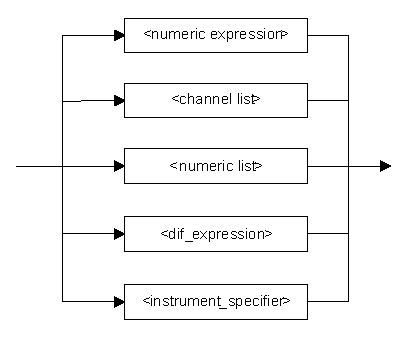
\includegraphics[scale=1]{Figuri/scpi_ro_3.eps}
 \caption{Sintaxa expresiilor}
 \label{fig5}
\end{figure}

\^{I}n cadrul expresiilor, "spa\c{t}iile albe" asa cum sunt denumite \^{i}n standardul IEEE 488.2, sunt permise \^{i}ntre orice elemente lexicale. Prin element lexical se \^{i}n\c{t}elege un operator, un semn de punctua\c{t}ie, cuv\^{a}nt cheie, tip de valoare.

\subsection{Expresii numerice}
O expresie numeric\u{a} este o colec\c{t}ie de termeni care evalueaz\u{a} un num\u{a}r, un vector sau un alt tip de informa\c{t}ie.

Sintaxa unei expresii numerice:
\begin{itemize}
	\item un operator numeric \textless numeric\_operator\textgreater;
	\item un operator numeric unar \textless unar\_numeric\_operator\textgreater;
	\item o variabil\u{a} \textless variable\textgreater sau \textless trace\_name\textgreater;
	\item o list\u{a} de canale \textless channel\_list\textgreater
\end{itemize}

\section{Raportarea st\u{a}rii}
Un dispozitiv SCPI trebuie s\u{a} includ\u{a} un registru de stare special - OPERation precum \c{s}i un registru de stare dat\u{a}/semnal QUEStionable \^{i}mpreun\u{a} cu condi\c{t}iile asociate, evenimente \c{s}i comenzi de activare.

De asemenea se stabilesc anumite cerin\c{t}e adi\c{t}ionale pentru instrumentele care suport\u{a} ori INSTrumente logice multiple ori modele de TRIGger cu posibilit\u{a}\c{t}i extinse. \^{I}n mod normal un registru de stare trebuie s\u{a} intre \^{i}ntr-o valoare \^{i}ntreag\u{a} de 16 bi\c{t}i cu bitul cel mai semnificativ totdeauna egal cu zero (logic pozitiv).
 % Introduction
% Chapter 1

\chapter{Lex \c{s}i Yacc} % Write in your own chapter title
\label{Capitolul3}
\lhead{Capitolul 3. \emph{Lex \c{s}i Yacc}} % Write in your own chapter title to set the page header

Lex este un generator de analizoare lexicale \c{s}i constituie unul dintre utilitarele standard ale sistemelor de operare Unix.

Programul \emph{lex} prime\c{s}te la intrare un fi\c{s}ier con\c{t}in\^{a}nd o specifica\c{t}ie a atomilor pe care urmeaz\u{a} s\u{a}-i recunoasc\u{a} analizorul generat, precum \c{s}i a ac\c{t}iunilor semantice de executat. Pe baza acestei specifica\c{t}ii se genereaz\u{a} un program C ce con\c{t}ine tabelele de analiz\u{a}, \^{i}mpreun\u{a} cu func\c{t}ia de analiz\u{a}, numit\u{a} \emph{yylex( )}. \^{I}n continuare se compileaz\u{a} programul ob\c{t}inut, rezult\^{a}nd astfel analizorul lexical executabil. 

Fi\c{s}ierul ce con\c{t}ine specifica\c{t}ia este un fi\c{s}ier text care poate avea orice nume acceptat de sistemul de operare. Se recomand\u{a} ca fi\c{s}ierul de specifica\c{t}ie s\u{a} aibe extensia \emph{.l}.

Programul C rezultat este memorat \^{i}ntr-un fi\c{s}ier denumit implicit lex.yy.c (utilizatorul poate solicita explicit un alt nume).  Efectuarea analizei lexicale asupra unui text surs\u{a} folosind analizorul generat de LEX este ilustrat\u{a} \^{i}n figura de mai jos.

\begin{figure}[htp]
 \centering
 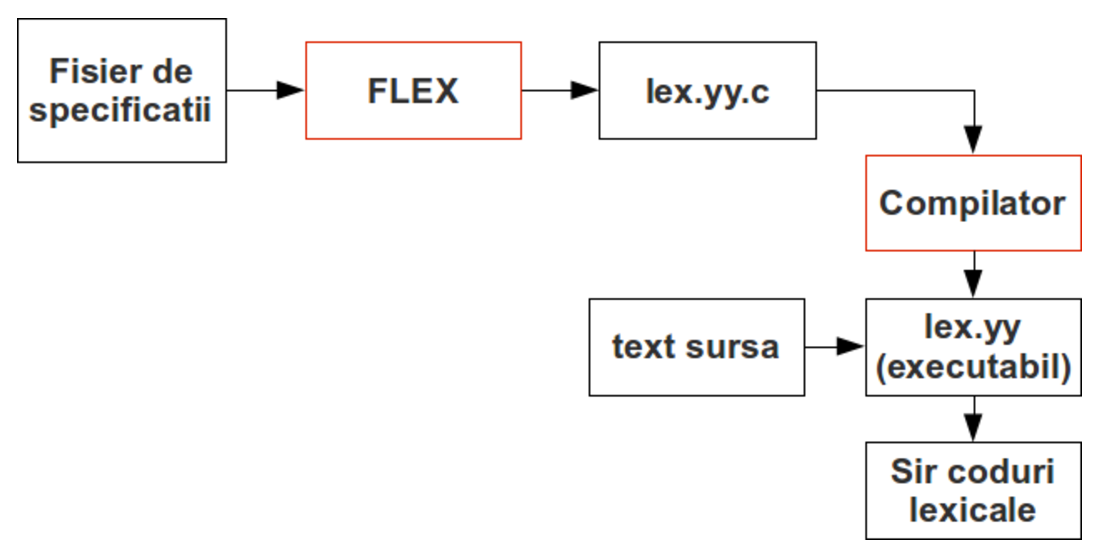
\includegraphics[scale=0.6]{Figuri/flex.eps}
 \caption{Analiza lexical\u{a} folosind Lex}
 \label{figflex}
\end{figure}

\section{Lansarea \^{i}n execu\c{t}ie a programului LEX}

Lansarea \^{i}n execu\c{t}ie a programului LEX se realizeaz\u{a} cu comanda
\begin{center}
lex [\emph{op\c{t}iuni}] [\emph{nume\_fi\c{s}ier\_specifica\c{t}ii}]
\end{center}
\^{I}n cazul \^{i}n care \emph{nume\_fi\c{s}ier\_specifica\c{t}ii} nu este precizat, LEX va a\c{s}tepta introducerea specifica\c{t}iilor de la stdin. 

C\^{a}teva dintre op\c{t}iunile liniei de comand\u{a} mai des utilizate sunt:
\begin{itemize}
	\item \emph{-d} = analizorul generat va func\c{t}iona \^{i}n regim "debug", adic\u{a} la fiecare atom recunoscut se va afi\c{s}a pe stderr un mesaj care con\c{t}ine num\u{a}rul liniei din fi\c{s}ierul de specifica\c{t}ii unde apare regula ata\c{s}at\u{a} atomului respectiv \c{s}i secven\c{t}a de caractere ce compun atomul; se precizeaz\u{a} c\u{a} efectul op\c{t}iunii \emph{-d} se ob\c{t}ine cu condi\c{t}ia ca variabila global\u{a} \emph{yy\_flex\_debug} s\u{a} fie setat\u{a} pe o valoare nenul\u{a}  (implicit variabila are valoarea 0);
	\item \emph{-h} = genereaz\u{a} la stdout un rezumat al op\c{t}iunilor din linia de comand\u{a} (-? \c{s}i --help au acela\c{s}i efect);
	\item \emph{-i} = analizorul generat va fi case-insensitiv (la identificatorii \c{s}i cuvintele cheie din textul surs\u{a} nu se va face distinc\c{t}ie \^{i}ntre literele mari \c{s}i cele mici);
	\item \emph{-o} = nume\_fi\c{s}ier\_ie\c{s}ire = aceast\u{a} op\c{t}iune se folose\c{s}te dac\u{a} se dore\c{s}te ca fi\c{s}ierul de ie\c{s}ire al generatorului s\u{a} aibe alt nume dec\^{a}t lex.yy.c;
	\item \emph{-T} = generatorul va lucra \^{i}n regim "trace", furniz\^{a}nd informa\c{t}ii utile care reflect\u{a} mersul procesului de construire a automatelor finite (nedeterminist \c{s}i determinist);
	\item \emph{-V} = la stdout se afi\c{s}eaz\u{a} versiunea programului LEX;
	\item \emph{-+} = analizorul generat va fi \^{i}n limbajul C++ (implicit el este \^{i}n ANSI-C).
\end{itemize}

Programul FLEX permite exprimarea unor op\c{t}iuni \c{s}i \^{i}n cadrul programului de specifica\c{t}ie \^{i}nsu\c{s}i, prin utilizarea directivei \emph{\%option} plasat\u{a} \^{i}n sec\c{t}iunea de defini\c{t}ii.

\section{Structura programului de specifica\c{t}ie}
Programul de specifica\c{t}ie con\c{t}ine \^{i}n principiu expresiile regulate ce descriu atomii limbajului surs\u{a}, precum \c{s}i ac\c{t}iunile pe care analizorul trebuie s\u{a} le execute la recunoa\c{s}terea fiec\u{a}rui atom.

Structura unui program de specifica\c{t}ie este urm\u{a}toarea:
\begin{verbatim}
sectiune definitii
%%
sectiune reguli
%%
cod utilizator
\end{verbatim}

\subsection{Sec\c{t}iunea de defini\c{t}ii}
Este utilizat\u{a} \^{i}n principal pentru a asocia nume expresiilor regulate, \^{i}n scopul ob\c{t}inerii unei specifica\c{t}ii mai simple \c{s}i mai clare.

\^{I}n afar\u{a} de aceasta, \^{i}n sec\c{t}iunea de defini\c{t}ii mai pot sa apar\u{a}:
\begin{itemize}
	\item directive \emph{\%option}
	\item declara\c{t}ii de st\u{a}ri de start
	\item secven\c{t}e C definite de utilizator
\end{itemize}
Pentru asocierea numelor cu expresiile regulate se utilizeaz\u{a} o construc\c{t}ie de forma:
\begin{center}
nume defini\c{t}ie
\end{center}
unde:
\begin{itemize}
	\item \textbf{nume} este un cuv\^{a}nt compus din una sau mai multe litere, cifre, '\_' sau '-', cu observa\c{t}ia c\u{a} primul caracter \emph{trebuie} s\u{a} fie liter\u{a} sau '\_' \c{s}i \emph{s\u{a} se afle pe prima pozi\c{t}ie a liniei};
	\item \textbf{defini\c{t}ie} este o expresie regulat\u{a} \c{s}i se consider\u{a} c\u{a} \^{i}ncepe cu primul caracter non-spa\c{t}iu de dup\u{a} nume \c{s}i \c{t}ine p\^{a}n\u{a} la sf\^{a}r\c{s}itul liniei.
\end{itemize}

Odat\u{a} declarat, un nume poate fi utilizat \^{i}n alte expresii regulate, sub forma:
\begin{center}
\{nume\}
\end{center}

Se poate considera c\u{a} numele asociate cu expresiile regulate sunt tratate \^{i}ntr-un mod similar directivelor \emph{\#define} dintr-un program C.

Directivele \emph{\%option} permit utilizatorului s\u{a} precizeze unele op\c{t}iuni legate de analizorul generat. C\^{a}teva asemenea op\c{t}iuni sunt:

\begin{itemize}
	\item \emph{\%option main} - are ca efect generarea unei func\c{t}ii main() care nu face altceva decat s\u{a} apeleze func\c{t}ia de analiz\u{a} yylex();
	\item \emph{\%option caseless} - are acela\c{s}i efect ca \c{s}i op\c{t}iunea -i din linia de comand\u{a};
	\item \emph{\%option debug} - are acela\c{s}i efect ca \c{s}i op\c{t}iunea -d din linia de comand\u{a}; 
	\item \emph{\%option yylineno} - analizorul rezultat va con\c{t}ine cod care actualizeaz\u{a} variabila global\u{a} yylineno cu valoarea curent\u{a} a num\u{a}rului liniei surs\u{a}; 
	\item \emph{\%option noyywrap} - aceast\u{a} op\c{t}iune este foarte util\u{a} dac\u{a} se dore\c{s}te ca la o rulare a analizorului s\u{a} se parcurg\u{a} un singur fi\c{s}ier surs\u{a}, a\c{s}a cum de fapt trebuie s\u{a} se \^{i}nt\^{a}mple de cele mai multe ori. 
\end{itemize}

Dac\u{a} aceast\u{a} op\c{t}iune lip\c{s}este, analizorul generat \^{i}ncearc\u{a} s\u{a} prelucreze \^{i}n lan\c{t} mai multe fi\c{s}iere surs\u{a}. Trecerea de la un fi\c{s}ier la altul se realizeaz\u{a} prin apelul de c\u{a}tre analizor a unei func\c{t}ii numite yywrap(), la \^{i}nt\^{a}lnirea marcajului EOF al fiec\u{a}rui fi\c{s}ier surs\u{a}. Cum func\c{t}ia yywrap() nu exist\u{a} \^{i}n mod implicit, ea ar trebui definit\u{a} de c\u{a}tre utilizator. Rolul acestei func\c{t}ii este s\u{a} deschid\u{a} urm\u{a}torul fi\c{s}ier \^{i}n variabila global\u{a} FILE *yyin \c{s}i s\u{a} returneze 0, respectiv s\u{a} returneze o valoare nenul\u{a} dac\u{a} nu mai exist\u{a} un fi\c{s}ier urm\u{a}tor.

Utilizatorul are posibilitatea de a plasa \^{i}n sec\c{t}iunea de defini\c{t}ii secven\c{t}e proprii de cod C. O modalitate de a introduce aceste secven\c{t}e C este ca ele s\u{a} fie incluse \^{i}ntre perechile de caractere \%\{ \c{s}i respectiv \%\}. Perechile \%\{ \c{s}i \%\} trebuie s\u{a} apar\u{a} pe linii separate \c{s}i neindentate. 

Codul cuprins \^{i}ntre aceste perechi (exclusiv perechile) va fi copiat ad-literam \^{i}n analizorul generat, \^{i}n spa\c{t}iul de vizibilitate din afara func\c{t}iei yylex(). Cu alte cuvinte, codul utilizator plasat \^{i}n sec\c{t}iunea de defini\c{t}ii va fi considerat ca spa\c{t}iu de declara\c{t}ii globale \^{i}n raport cu func\c{t}ia yylex().

\^{I}ntruc\^{a}t orice linie indentat\u{a} din sec\c{t}iunea de defini\c{t}ii este copiat\u{a} f\u{a}r\u{a} modific\u{a}ri \^{i}n analizorul generat, rezult\u{a} c\u{a} perechile delimitatoare \%\{ \c{s}i \%\} pot lipsi, cu condi\c{t}ia ca toate liniile de cod ale utilizatorului s\u{a} fie scrise indentat. 

\subsection{Sec\c{t}iunea de reguli}

Scopul principal al acestei sec\c{t}iuni este acela de a asocia ac\c{t}iuni semantice cu expresiile regulate. \^{I}n plus, ea mai poate con\c{t}ine cod C definit de utilizator.

Pentru asocierea ac\c{t}iunilor semantice cu expresiile regulate se utilizeaz\u{a} o construc\c{t}ie de forma:
\begin{center}
\c{s}ablon ac\c{t}iune
\end{center}
unde:
\begin{itemize}
	\item \textbf{\c{s}ablon} este o expresie regulat\u{a}, al c\u{a}rei prim caracter \emph{trebuie s\u{a} se afle pe prima pozi\c{t}ie a liniei};
	\item \textbf{ac\c{t}iune} este o secven\c{t}\u{a} format\u{a} din una sau mai multe instruc\c{t}iuni C care \emph{trebuie s\u{a} \^{i}nceap\u{a} pe aceea\c{s}i linie cu \c{s}ablonul}. Dac\u{a} secven\c{t}a e format\u{a} din mai multe instruc\c{t}iuni, acestea se vor \^{i}nchide \^{i}ntre acolade. \^{I}n particular, ac\c{t}iunea poate fi \c{s}i instruc\c{t}iunea vid\u{a}.
\end{itemize}

Semnifica\c{t}ia unei asemenea construc\c{t}ii este c\u{a} analizorul generat va executa secven\c{t}a descris\u{a} ca ac\c{t}iune atunci c\^{a}nd va recunoa\c{s}te \^{i}n textul surs\u{a} un \c{s}ir care se potrive\c{s}te cu \c{s}ablonul. 

Dac\u{a} ac\c{t}iunea este redat\u{a} prin instruc\c{t}iunea vid\u{a}, la recunoa\c{s}terea \c{s}irului descris de \c{s}ablonul \^{i}n cauz\u{a}, analizorul nu va executa nimic (de fapt, va trece pur \c{s}i simplu la delimitarea urm\u{a}torului atom). \^{I}n consecin\c{t}\u{a}, atomii ale c\u{a}ror reguli au ac\c{t}iune vid\u{a} sunt neglija\c{t}i (filtra\c{t}i sau elimina\c{t}i). Comentariile \c{s}i spa\c{t}iile albe sunt exemple de \c{s}iruri care se preteaz\u{a} la un asemenea tratament.

Dac\u{a} o ac\c{t}iune se termin\u{a} cu instruc\c{t}iunea return, aceasta va \^{i}nsemna ie\c{s}irea din func\c{t}ia yylex(), altfel aceast\u{a} func\c{t}ie trece automat la c\u{a}utarea urm\u{a}toarelor potriviri. \^{I}n concluzie, dac\u{a} dorim ca analizorul lexical s\u{a} prelucreze c\^{a}te un singur atom la fiecare apel, va trebui s\u{a} prevedem instruc\c{t}iuni return la toate ac\c{t}iunile care corespund unor atomi valizi (nu comentarii sau spa\c{t}ii albe). Acest mod de lucru este potrivit pentru compilatoarele care lucreaz\u{a} \^{i}ntr-o singur\u{a} trecere. Pentru compilatoarele care lucreaz\u{a} \^{i}n mai multe treceri, analiza lexical\u{a} fiind o faz\u{a} distinct\u{a}, ac\c{t}iunile se vor termina prin instruc\c{t}iuni de scriere (de exemplu directiva ECHO) a codurilor lexicale \^{i}ntr-un fi\c{s}ier de ie\c{s}ire (care ar putea fi yyout). 

\paragraph{Exemple de variabile utile:}
\begin{itemize}
	\item char *yytext - reprezint\u{a} adresa zonei de memorie \^{i}n care se depun caracterele ce compun atomul curent;
	\item int yyleng - reprezint\u{a} lungimea atomului curent;
	\item FILE *yyin - desemneaz\u{a} fi\c{s}ierul care con\c{t}ine textul surs\u{a} de analizat;
	\item FILE *yyout - desemneaz\u{a} fi\c{s}ierul \^{i}n care se poate scrie cu ajutorul macro-ului ECHO.
\end{itemize}

\paragraph{Exemple de macrouri \c{s}i func\c{t}ii utile:}
\begin{itemize}
	\item ECHO - realizeaz\u{a} scrierea con\c{t}inutului zonei yytext \^{i}n fi\c{s}ierul desemnat prin yyout;
	\item BEGIN nume\_stare\_start - realizeaz\u{a} comutarea analizorului \^{i}n starea de start specificat\u{a};
	\item REJECT - caut\u{a} urm\u{a}toarea regul\u{a} a c\u{a}rei \c{s}ablon se potrive\c{s}te cu atomul \^{i}n curs de prelucrare, sau cu un prefix al acestuia, \c{s}i execut\u{a} ac\c{t}iunea asociat\u{a} regulii g\u{a}site;
	\item YY\_START - furnizeaz\u{a} starea de start curent\u{a} (o valoare \^{i}ntreag\u{a});
	\item yyterminate() - are ca efect terminarea procesului de analiza \c{s}i returnarea valorii 0 c\u{a}tre apelantul func\c{t}iei yylex(); yyterminate() este un macro \c{s}i poate fi redefinit\u{a} de utilizator;
	\item void yymore() - determin\u{a} concatenarea urm\u{a}torului atom din textul surs\u{a} la atomul existent \^{i}n yytext (\^{i}n mod normal, urm\u{a}torul atom \^{i}l \^{i}nlocuie\c{s}te pe cel precedent);
	\item void yyless(int n) - las\u{a} \^{i}n yytext primele n caractere ale atomului curent, restituind \^{i}n \c{s}irul de intrare caracterele de pe pozi\c{t}iile n+1 p\^{a}n\u{a} la sf\^{a}r\c{s}it; actualizeaz\u{a} apoi valoarea lui yylen la n (caracterele restituite vor fi analizate ulterior);
	\item void unput(char c) - for\c{t}eaza plasarea \^{i}n \c{s}irul de intrare a caracterului c, acesta devenind urm\u{a}torul caracter de analizat;
	\item int input() - cite\c{s}te \c{s}i returneaz\u{a} urm\u{a}torul caracter din \c{s}irul de intrare.
\end{itemize}

\section{Expresii regulate}

Prima etap\u{a} \^{i}n \^{i}n\c{t}elegerea unui program este descompunerea lui \^{i}n lexeme. Se nume\c{s}te lexem\u{a}, un \c{s}ir de caractere de la intrare care este \^{i}n curs de analizare. 

De exemplu, \^{i}n C avem lexeme de forma for, while, etc., dar nu lexeme de forma \%\$\#@.

\^{I}n plus, \^{i}n C putem \^{i}nt\^{a}lni lexeme de genul variabila\_cea\_mare. Exist\u{a} deci un numar poten\c{t}ial infinit de lexeme (dac\u{a} presupunem c\u{a} numele de variabile nu au nicio limit\u{a} pentru lungime).

Teoreticienii au propus \^{i}n anii 1960 un meta-limbaj extrem de concis pentru a descrie lexeme. Limbajul acesta este limbajul expresiilor regulate. O expresie regulat\u{a} este un \c{s}ir de caractere care descrie o mul\c{t}ime de cuvinte posibile (poate chiar o mul\c{t}ime infinit\u{a}). Lexemele tuturor limbajelor de programare moderne pot fi descrise prin expresii regulate.

Pe baza expresiilor regulate se poate construi un automat cu st\u{a}ri finite, care st\u{a} la baza func\c{t}ionarii unui analizor lexical. Un automat cu st\u{a}ri finite este o ma\c{s}ina abstract\u{a} care poate analiza \c{s}i recunoa\c{s}te expresiile regulate, iar implementarea software a unui astfel de automat nu este dificil\u{a}.

Folosind expresiile regulate, se poate defini o gramatic\u{a} de expresii pentru un limbaj surs\u{a}.

Semnifica\c{t}ia expresiilor regulate:
\begin{itemize}
	\item . - semnific\u{a} orice caracter cu excep\c{t}ia lui newline;
	\item * - semnific\u{a} zero sau mai multe apari\c{t}ii ale expresiei regulate precedente;
	\item {[}{]} - semnific\u{a} o clas\u{a} de caractere;
	\item \^ - un circumflex la \^{i}nceputul unei expresii regulate semnific\u{a} faptul c\u{a} expresia respectiv\u{a} trebuie s\u{a} apar\u{a} chiar la \^{i}nceputul unei linii \^{i}n limbajul surs\u{a};
	\item \$ - un dolar la \^{i}nceputul unei expresii regulate semnific\u{a} faptul c\u{a} expresia respectiv\u{a} trebuie s\u{a} apar\u{a} chiar la sfar\c{s}itul unei linii \^{i}n limbajul surs\u{a};
	\item \{\} - indic\u{a} un domeniu restr\^{a}ns de copii ale expresiei regulate precedente. De exemplu, (abc)\{3,8\} semnific\u{a} \^{i}ntre 3 \c{s}i 8 apari\c{t}ii ale cuvantului 'abc';
	\item + - semnific\u{a} una sau mai multe apari\c{t}ii ale expresiei regulate precedente;
	\item ? - semnific\u{a} zero sau o singur\u{a} apari\c{t}ie a expresiei regulate precedente;
	\item \textbar - expresia regulat\u{a} precedent\u{a}, sau expresia regulat\u{a} urm\u{a}toare;
	\item "..." - tot ce este cuprins \^{i}ntre ghilimele se interpreteaz\u{a} literal;
	\item () - grupeaz\u{a} o serie de expresii regulate \^{i}ntr-o expresie nou\u{a}.
\end{itemize}

\section{Utilizarea generatorului de parsere Yacc}
Yacc poate genera un traducator \^{i}n modul urm\u{a}tor: specifica\c{t}iile sintactice precum \c{s}i unele elemente semantice sunt incluse \u{i}ntr-un fi\c{s}ier de intrare pentru Yacc. Acest fi\c{s}ier are \^{i}n general extensia ".y". Linia de comanda (in UNIX):
\begin{center}
yacc nume\_fisier.y
\end{center}
produce, plec\^{a}nd de la specifica\c{t}iile cuprinse \^{i}n fi\c{s}ierul de intrare nume\_fi\c{s}ier.y, un program scris \^{i}n limbaj C care implementeaz\u{a} metoda de analiz\u{a} sintactica LARL pentru gramatica respectiv\u{a} - \^{i}n spe\c{t}\u{a} func\c{t}ia yyparse(). Fi\c{s}ierul de intrare (programul surs\u{a}) pentru Yacc are structura urm\u{a}toare:
\begin{verbatim}
Declaratii
%%
Reguli
%%
Rutine C
\end{verbatim}

Partea Declara\c{t}ii a fi\c{s}ierului surs\u{a} este op\c{t}ional\u{a} \c{s}i poate cuprinde dou\u{a} sec\c{t}iuni. O prim\u{a} sec\c{t}iune cuprinde \^{i}ntre delimitatorii \%\{ \c{s}i \%\} declara\c{t}ii \^{i}n limbajul C pentru variabilele care se utilizeaz\u{a} \^{i}n regulile de traducere sau \^{i}n procedurile din cea de-a treia parte a fi\c{s}ierului. A\c{s}adar, textul cuprins \^{i}ntre \%\{ \c{s}i \%\} se copie nealterat \^{i}n fi\c{s}ierul C produs de Yacc. A doua sec\c{t}iune a acestei prime p\u{a}rti con\c{t}ine declara\c{t}ii ale unit\u{a}\c{t}ilor lexicale ale gramaticii, declara\c{t}ii de asociativitate \c{s}i preceden\c{t}\u{a} a operatorilor, declara\c{t}ii ale tipurilor de date pentru valorile semantice ale simbolurilor gramatacii.

Simbolurile terminale ale gramaticii,cu excep\c{t}ia celor formate dintr-un singur caracter (precum +, * etc), trebuiesc declarate. Aceste simboluri sunt reprezentate \^{i}n Yacc prin ni\c{s}te coduri numerice; func\c{t}ia yylex transmite codul unit\u{a}\c{t}ii respective func\c{t}iei yyparse. Programatorul nu trebuie s\u{a} \c{s}tie aceste coduri numerice, ele sunt generate automat folosind op\c{t}iunea -d la lansarea Yacc \c{s}i sunt trecute \^{i}ntr-un fi\c{s}ier nume.tab.h (sau yytab.h sub DOS). Unit\u{a}\c{t}ile lexicale se definesc prin linii de forma:
\begin{verbatim}
% token <nume_unitate_lexicala>
\end{verbatim}
\c{s}i pot fi utilizate \^{i}n celelalte dou\u{a} par\c{t}i ale fi\c{s}ierului de intrare. Tot \^{i}n aceast\u{a} sec\c{t}iune se poate introduce simbolul de start al gramaticii, \^{i}n cazul \^{i}n care aceasta nu este partea st\^{a}nga a primei reguli sintactice:
\begin{verbatim}
start <nume_simbol_de_start>
\end{verbatim}

Alte linii care pot fi incluse \^{i}n aceast\u{a} sec\c{t}iune sunt:
\begin{itemize}
	\item type - pentru definirea tipului;
	\item left - pentru asociativitate st\^{a}nga a operatorilor;
	\item right - pentru asociativitate dreapta a operatorilor;
	\item prec - pentru precizarea preceden\c{t}ei operatorilor;
	\item nonassoc - pentru declara\c{t}iile de neasociativitate.
\end{itemize}

Simbolurile gramaticii pot avea valori semantice. \^{I}n mod implicit, aceste valori sunt valori \^{i}ntregi \c{s}i sunt specificate \^{i}n YYSTYPE. Pentru a specifica alt tip, \^{i}n partea de declara\c{t}ii C se adaug\u{a} o directiv\u{a} define pentru YYSTYPE:
\begin{verbatim}
#define YYSTYPE <nume tip>
\end{verbatim}

Utilizarea de tipuri diferite pentru simboluri diferite se realizeaz\u{a} prin specificarea acestor tipuri \^{i}ntr-o declara\c{t}ie union (specific\u{a} Yacc) \c{s}i declararea tipului simbolurilor cu type. Iat\u{a} un exemplu:
\begin{verbatim}
%union {
	int intval;
	double doubleval;
	symrec *tptr;
}
type <intval> INT
type <doubleval> REAL
type <tptr> ID
\end{verbatim}

Prin aceste declara\c{t}ii se specific\u{a} tipul valorilor pentru token-urile INT, REAL, ID ca fiind respectiv int, double, pointer la symrec (pointer \^{i}n tabela de simboluri).

Partea a doua a fi\c{s}ierului de intrare, \emph{Reguli}, este partea obligatorie. Aici se specific\u{a} regulile gramaticii care descriu sintaxa pe care dorim s\u{a} o verificam cu acest analizor. Fiecare regul\u{a} con\c{t}ine:
\begin{itemize}
	\item partea st\^{a}ng\u{a};
	\item partea dreapt\u{a};
	\item partea de ac\c{t}iune.
\end{itemize}

Partea st\^{a}ng\u{a} trebuie s\u{a} con\c{t}in\u{a} un neterminal al gramaticii, iar partea dreapt\u{a} \c{s}irul format din terminali \c{s}i neterminali, corespunz\u{a}tor unei reguli. Cele dou\u{a} p\u{a}r\c{t}i sunt desp\u{a}r\c{t}ite prin ":". Partea de ac\c{t}iune, cuprins\u{a} \^{i}ntre \{ \c{s}i \}, con\c{t}ine un text scris \^{i}n limbajul C care va fi inclus \^{i}n analizor \c{s}i reprezint\u{a} opera\c{t}iile care se execut\u{a} atunci c\^{a}nd analizorul realizeaz\u{a} o reducere cu regula specificat\u{a}. O regul\u{a} se termin\u{a} prin ";". Dac\u{a} sunt mai multe reguli care au aceea\c{s}i parte st\^{a}nga, acestea se scriu o singura dat\u{a} \c{s}i par\c{t}ile drepte se despart prin "\textbar". Iat\u{a}, spre exemplu, cum se scriu regulile gramaticii care descrie expresiile aritmetice:
\begin{verbatim}
expr : NUMAR
| expr '+' expr
| expr '-' expr
| expr '*' expr
| expr '/' expr
| '(' expr ')'
;
\end{verbatim}

Aici, expr este numele neterminalului care define\c{s}te expresia aritmetic\u{a}, terminalii +, -, *, /, (, ) se pun \^{i}ntre apostrof, iar NUMAR reprezint\u{a} token-ul num\u{a}r. Dac\u{a} dorim ca analizorul pe care \^{i}l contruim s\u{a} realizeze \c{s}i ac\c{t}iuni semantice, de pild\u{a} s\u{a} evalueze expresiile, se adug\u{a} la reguli partea de ac\c{t}iune:
\begin{verbatim}
expr : NUMAR {$$ = $1;}
| expr '+' expr {$$ = $1+$3;}
| expr '-' expr {$$ = $1-$3;}
| '(' expr ')' {$$ = $2;}
;
\end{verbatim}

\^{I}n partea de ac\c{t}iune se scriu instruc\c{t}iuni \^{i}n limbajul C. Aici, \$\$ reprezint\u{a} valoarea unui atribut al neterminalului expr din st\^{a}nga regulii sintactice, iar \$i reprezint\u{a} valoarea atributului celui de-al i-lea simbol din partea st\^{a}nga a reguluii.

Ultima parte a fi\c{s}ierului de intrare con\c{t}ine rutine scrise \^{i}n limbaj C care se includ nealterate \^{i}n analizorul ob\c{t}inut de Yacc. \^{I}n aceast\u{a} parte trebuie furnizat un analizor lexical, adic\u{a} o func\c{t}ie yylex() precum \c{s}i apelul la func\c{t}ia yyparse() pe care o creeaz\u{a} Yacc.

\section{YACC: Recursivitatea \c{s}i ambiguitatea}
La specificarea unei liste, acest lucru se poate face fie folosind recursivitatea st\^{a}nga:
\begin{verbatim}
list : list ',' item { ... }
 | item { ... }
\end{verbatim}
fie folosind recursivitatea dreapta:
\begin{verbatim}
list : item ',' list { ... }
 | item { ... }
\end{verbatim}

Dac\u{a} folosim recursivitatea dreapta, toate elementele din list\u{a} sunt puse \^{i}n stiv\u{a}. Dup\u{a} ce ultimul item este introdus, abia atunci se \^{i}ncepe reducerea acestora. \^{I}n cazul recursivit\u{a}\c{t}ii st\^{a}nga, niciodat\u{a} nu vom avea mai mult de trei elemente \^{i}n stiv\u{a}, deoarece la fiecare trei se poate realiza o reducere, pe m\u{a}sur\u{a} ce ace\c{s}tia sunt furniza\c{t}i de scanner. Din acest motiv, este recomandat\u{a} folosirea recursivit\u{a}\c{t}ii st\^{a}nga.

Un conflict ce apare frecvent este acela al construc\c{t}iilor de tip if-then-else. S\u{a} consider\u{a}m c\u{a} avem urm\u{a}toarele produc\c{t}ii:

\begin{verbatim}
stmt : IF expr THEN stmt
 | IF expr THEN stmt ELSE stmt
 ...
\end{verbatim}
\c{s}i urm\u{a}torul context (unde am marcat cu . locul unde am ajuns cu parcurgerea instruc\c{t}iunii curente):

\begin{verbatim}
IF expr THEN stmt IF expr THEN stmt . ELSE stmt
\end{verbatim}

Trebuie s\u{a} decidem dac\u{a} shift\u{a}m ELSE sau reducem contextul IF expr THEN stmt care se afl\u{a} deja pe v\^{a}rful stivei. Limbajele de programare precizeaz\u{a} c\u{a} ELSE apar\c{t}ine celui mai inferior IF, deci trebuie \^{i}n acest caz s\u{a} realiz\u{a}m un shift. Aceast\u{a} ambiguitate se rezolv\u{a} acord\^{a}nd construc\c{t}iei if-then-else o preceden\c{t}\u{a} mai mare dec\^{a}t celei simple if-then:

\begin{verbatim}
%nonassoc IF_SIMPLU
%nonassoc ELSE

stmt : IF expr THEN stmt %prec IF_SIMPLU
 | IF expr THEN stmt ELSE stmt
\end{verbatim}

Acela\c{s}i tip de construc\c{t}ie se utilizeaz\u{a} \c{s}i la definirea preceden\c{t}ei produc\c{t}iei ata\c{s}ate minusului unar, de exemplu.

\section{Exemplu lex si yacc}
S\u{a} lu\u{a}m ca exemplu realizarea unui parser care s\u{a} recunoasc\u{a} toate \c{s}irurile limbajului:
\begin{equation}
 L=\left \{ w \mid w = a^{n}b^{n}, n\geqslant 0 \right \}
\end{equation} 
Gramatica acestui limbaj este:
\begin{verbatim}
A -> a A b | ab
\end{verbatim}

unde A este unicul neterminal \c{s}i \^{i}n acela\c{s}i timp simbol de start iar terminalii (tokenii) gramaticii sunt a \c{s}i b.

Vom scrie mai \^{i}nt\^{a}i scannerul ce recunoa\c{s}te tokenii limbajului dat. Acesta este urm\u{a}torul:
\begin{verbatim}
%{
#include "ex1.tab.h"
%}

%%

a	{return TOKEN_A;}
b	{return TOKEN_B;}
\.	{return yytext[0];}
.	{printf("tokenul %s nu este cunoscut\n", yytext);}
\n	{return yytext[0];}

%%
\end{verbatim}

Sec\c{t}iunea de defini\c{t}ii include fi\c{s}ierul ex1.tab.h ce va fi generat de yacc \c{s}i con\c{t}ine declara\c{t}iile tokenilor limbajului (TOKEN\_A \c{s}i TOKEN\_B).

Prima regul\u{a} din sec\c{t}iunea a doua specific\u{a} faptul c\u{a} fiecare apari\c{t}ie a caracterului "a" \^{i}n textul surs\u{a} reprezint\u{a} TOKEN\_A. La fel pentru cea de-a doua, care se refer\u{a} la "b". Cea de-a treia recunoa\c{s}te punctul. La \^{i}nt\^{a}lnirea lui, scannerul il recunoa\c{s}te \c{s}i \^{i}l paseaz\u{a} parser-ului ca atare, f\u{a}r\u{a} a-i asocia vreun cod. Cea de-a patra regul\u{a} se potrive\c{s}te tuturor celorlalte caractere recunoscute la intrare, iar ac\c{t}iunea asociat\u{a} afi\c{s}eaz\u{a} un mesaj de eroare. Aceasta nu se termin\u{a} cu "return", astfel scannerul p\u{a}streaza mai departe controlul - adic\u{a} tokenul recunoscut de aceast\u{a} regul\u{a} este ignorat de parser. \^{I}n fine, ultima regul\u{a} recunoa\c{s}te caracterul "newline" \c{s}i \^{i}l transmite ca atare parserului.

Sec\c{t}iunea de subrutine nu con\c{t}ine nimic \^{i}n cazul specific\u{a}rii scannerului.

Regulile gramaticii sunt precizate de fi\c{s}ierul ex1.y. Parserul are o procesare orientat\u{a} pe linii. Vom mai \^{i}mbog\u{a}\c{t}i gramatica astfel:

\begin{verbatim}
%token TOKEN_A TOKEN_B

%%

S : S T '\n'	{printf("n = %d\n", $2);}
 | S '\n'		{ /* linie goala testata */ }
 | S '.'		{return;}
 |				/* regula implicita */
 ;

T : TOKEN_A T TOKEN_B	{ $$ = $2 + 1; }
 | TOKEN_A TOKEN_B		{ $$ = 1; }
 ;
 
%%

int main(void)
{
	yyparse();
	return 0;
}

int yyerror(char *s)
{
	printf("%s\n", s);
}
\end{verbatim}

Prima sec\c{t}iune con\c{t}ine defini\c{t}iile tokenilor. Cea de-a doua descrie gramatica, ce are \^{i}n cazul ales \c{s}ase produc\c{t}ii. Simbolul de start este S. Deoarece el are o produc\c{t}ie lambda, aceasta este redus\u{a} implicit, adic\u{a} f\u{a}r\u{a} a citi nimic de la intrare, parserul \^{i}l va plasa pe S pe varful stivei. Pentru prima produc\c{t}ie a lui S, se detecteaz\u{a} o linie complet\u{a} ce con\c{t}ine un cuvant din limbajul specificat, deci se poate afi\c{s}a n. \$2 indic\u{a} valoarea celui de-al doilea neterminal din partea dreapt\u{a}, care este T, adic\u{a} un cuv\^{a}nt al limbajului. A doua produc\c{t}ie a lui S precizeaz\u{a} ac\c{t}iunea de realizat atunci c\^{a}nd se introduce o linie vid\u{a} (dac\u{a} se introduce "newline" \c{s}i pe stiv\u{a} nu era decat S, atunci acest neterminal se pastreaz\u{a}). A treia produc\c{t}ie pentru S va executa "return" din analizorul sintactic atunci c\^{a}nd utilizatorul introduce caracterul punct, adic\u{a} procesarea se \^{i}ncheie.

Produc\c{t}iile pentru T sunt relativ familiare. Ac\c{t}iunile de urmat sunt \^{i}ns\u{a} interesante. Astfel, pentru a doua produc\c{t}ie a lui T, se detecteaz\u{a} un nucleu ab, iar valoarea asociat\u{a} neterminalului rezultat al reducerii acestui \c{s}ir este 1. Prima regul\u{a} recunoa\c{s}te recursiv \c{s}iruri de dimensiuni din ce \^{i}n ce mai mari, iar valoarea neterminalului la care se reduce contextul recunoscut se calculeaz\u{a} prin incrementarea valorii neterminalului \^{i}ncadrat \^{i}ntre un a \c{s}i un b ce constituie handle-ul.

Sec\c{t}iunea de subrutine define\c{s}te func\c{t}ia main precum \c{s}i func\c{t}ia yyparse de tratare a erorilor de sintax\u{a}.
 % Introduction
% Chapter 1

\chapter{Implementare} % Write in your own chapter title
\label{Capitolul4}
\lhead{Capitolul 4. \emph{Implementare}} % Write in your own chapter title to set the page header

\section{Generatorul de semnal BK4070}

Modelul BK4070 este o surs\u{a} de semnal capabil\u{a} s\u{a} genereze o varietate de forme de und\u{a}. Panoul frontal prezint\u{a} doi conectori de ie\c{s}ire. Conectorul SIG Out este principala ie\c{s}ire de semnal. Conectorul SYNC Out este o ie\c{s}ire de semnal dreptunghiular compatibil TTL/CMOS. Acest semnal este de +5V \c{s}i este util pentru comanda diverselor circuite digitale.

Unitatea dispune de asemenea de un conector RS-232 pe panoul din spate. Acesta permite utilizatorului s\u{a} controleze de la distan\c{t}a generatorul, utiliz\^{a}nd caractere ASCII. Nu sunt necesare componente sau protocoale speciale; orice terminal sau port serial de calculator pot fi utilizate. Viteza este reglabil\u{a}, p\^{a}n\u{a} la 115.2 Kbps. 

\section{Comenzile de control la distan\c{t}\u{a}}
Diagrama de mai jos prezint\u{a} tastele de pe panoul frontal \c{s}i codurile ASCII asociate lor. Trimiterea acestor caractere la BK4070 are acela\c{s}i efect ca \c{s}i ap\u{a}sarea butonului de pe panoul frontal.
\begin{figure}[!htb]
	\centering
	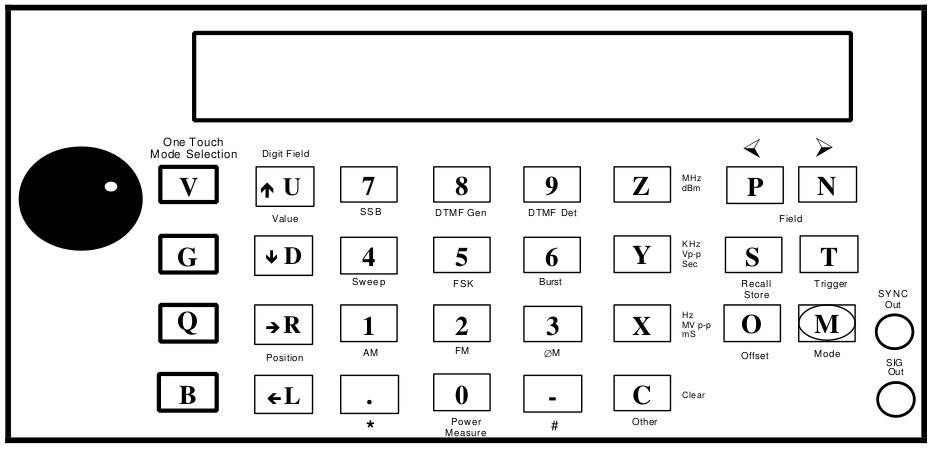
\includegraphics[scale=0.4]{panoufrontal.jpg}
	\caption{Tastele \c{s}i caracterele ASCII echivalente de pe panoul frontal}
	\label{panoufrontal}
\end{figure}

\^{I}n plus fa\c{t}\u{a} de comenzile \^{i}n caractere ASCII, sunt disponibile comenzi suplimentare pentru opera\c{t}iuni de control de la distan\c{t}\u{a}. Acestea sunt:
\begin{itemize}
	\item A - reseteaz\u{a} aparatul la modul semnal sinusoidal;
	\item V - furnizeaz\u{a} versiunile hardware \c{s}i software;
	\item K1,0 - Activeaz\u{a}, Dezactiveaz\u{a} tastele de pe panoul frontal;
	\item E1,0 - Activeaz\u{a}, Dezactiveaz\u{a} transmiterea c\u{a}tre terminal a textului de pe LCD;
	\item F0-9 - Mut\u{a} cursorul la c\^{a}mpurile 0-9;
	\item ? sau H - afi\c{s}eaz\u{a} meniul Help;
	\item \textasciicircum E - returneaz\u{a} \textasciicircum C.
\end{itemize}

Exemplu:
\begin{verbatim}
B F1 3.141Z N 2.3Z F0
\end{verbatim}
\begin{itemize}
	\item B - seteaz\u{a} aparatul \^{i}n modul semnal sinusoidal;
	\item F1 - mut\u{a} cursorul la c\^{a}mpul 1;
	\item 3.141Z - valoarea frecven\c{t}ei de 3.141 MHz;
	\item N - mut\u{a} cursorul la urm\u{a}torul c\^{a}mp;
	\item 2.3Z - valoarea de +2.3 dBm;
	\item F0 - mut\u{a} cursorul la c\^{a}mpul 0.
\end{itemize}

\section{Modul Basic Sinewave}
Acest mod genereaz\u{a} semnal sinusoidal de o anumit\u{a} frecven\c{t}\u{a}. Cei doi parametri necesari sunt Frecven\c{t}a \c{s}i Nivelul.

Pentru generarea unui semnal sinusoidal de 5000 KHz, 4 Vp-p, comanda va fi:

\begin{verbatim}B F1 5000X F2 4Y \end{verbatim}

Comenzile SCPI echivalente sunt:
\begin{verbatim}
SOURce:FREQuency 5000
SOURce:VOLTage 4
FUNCtion SINusoid
\end{verbatim}

\section{Modul Internal AM}
Acest mod genereaz\u{a} semnal modulat \^{i}n amplitudine folosindu-se un semnal sinusoidal generat intern ca semnal modulator. Parametrii necesari sunt Frecven\c{t}a de modulare, Procentul modula\c{t}iei, Frecven\c{t}a purt\u{a}toarei \c{s}i Nivelul PEP.

Exemplu:
\begin{verbatim}
M1 1 F1 4000X F2 40Z F3 5000X F4 3Y
\end{verbatim}

Echivalentul SCPI:
\begin{verbatim}
SOURce:FREQuency 5000
SOURce:VOLTage 3
SOURce:AM:SOURce INTernal
SOURce:AM:DEPTh 40
SOURce:AM:INTernal:FREQuency 4000
SOURce:AM:STATe ON
\end{verbatim}

\section{Modul External AM}
Acest mod genereaz\u{a} semnal modulat \^{i}n amplitudine folosindu-se ca semnal modulator un semnal exterior. Parametrii necesari sunt Input Gain, Frecven\c{t}a purt\u{a}toarei, Nivel PEP.

Exemplu:
\begin{verbatim}
M1 2 F1 0Z F2 5000X F3 3Y
\end{verbatim}

Exhivalentul SCPI:
\begin{verbatim}
SOURce:FREQuency 5000
SOURce:VOLTage 3
SOURce:AM:SOURce EXTernal
SOURce:AM:STATe ON
\end{verbatim}

\section{Modul Internal FM}
Acest mod genereaz\u{a} semnal modulat \^{i}n frecven\c{t}\u{a}, folosindu-se de un semnal generat intern. Parametrii necesari sunt Frecven\c{t}a de modulare, Peak Frequency Deviation, Frecven\c{t}a purt\u{a}toarei \c{s}i Nivel.

Exemplu:
\begin{verbatim}
M2 1 F1 3000X F2 4000X F3 5000X F4 4Y
\end{verbatim}

Echivalent SCPI:
\begin{verbatim}
SOURce:FREQuency 5000
SOURce:VOLTage 4
SOURce:FM:SOURce INTernal
SOURce:FM:INTernal:FREQuency 3000
SOURce:FM:DEViation 4000
SOURce:FM:STATe ON
\end{verbatim}

\section{Modul External FM}
Acest mod genereaz\u{a} semnal modulat \^{i}n frecven\c{t}\u{a}, folosindu-se de un semnal extern. Parametrii necesari sunt Peak Frequency Deviation, Frecven\c{t}a purt\u{a}toarei \c{s}i Nivel.

Exemplu:
\begin{verbatim}
M2 2 F1 4000X F2 5000X F3 4Y
\end{verbatim}

Echivalent SCPI:
\begin{verbatim}
SOURce:FREQuency 5000
SOURce:VOLTage 4
SOURce:FM:SOURce EXTernal
SOURce:FM:DEViation 4000
SOURce:FM:STATe ON
\end{verbatim}

\section{Modul Internal PM}
Acest mod genereaz\u{a} semnal modulat \^{i}n faz\u{a} de amplitudine fix\u{a}. Acesta utilizeaz\u{a} semnal generat intern pentru a modula faza semnalului purt\u{a}tor. Parametrii necesari sunt Frecven\c{t}a de modulare, Peak Phase Deviation, Frecven\c{t}a purt\u{a}toarei \c{s}i Nivel.

Exemplu:
\begin{verbatim}
M3 1 F1 4000X F2 3000 F3 3000X F4 4Y
\end{verbatim}

Echivalent SCPI:
\begin{verbatim}
SOURce:FREQuency 3000
SOURce:VOLTage 4
SOURce:PM:SOURce INTernal
SOURce:PM:INTernal:FREQuency 4000
SOURce:PM:DEViation 3000
SOURce:PM:STATe ON
\end{verbatim}

\section{Modul External PM}
Acest mod genereaz\u{a} semnal modulat \^{i}n faz\u{a} de amplitudine fix\u{a}, unde un semnal modulator extern este folosit pentru varierea fazei semnalului purt\u{a}tor. Parametrii necesari sunt Peak Phase Deviation, Frecven\c{t}a purt\u{a}toarei, Nivel.

Exemplu:
\begin{verbatim}
M3 2 F1 4000X F2 3000X F3 4Y
\end{verbatim}

Echivalent SCPI:
\begin{verbatim}
SOURce:FREQuency 3000
SOURce:VOLTage 4
SOURce:PM:SOURce EXTernal
SOURce:PM:DEViation 4000
SOURce:PM:STATe ON
\end{verbatim}

\section{Modul Sweep}
Acest mod schimb\u{a} continuu frecven\c{t}a unui semnal sinusoidal de amplitudine fix\u{a} \^{i}n intervalul frecven\c{t}\u{a} de start \c{s}i stop specificate. Parametrii necesari sunt Frecven\c{t}a de start, Frecven\c{t}a de stop, Liniar/Logaritmic, Continuu/Triggerat, Up/Down, Timp de sweep \c{s}i Nivel.

Exemplu:
\begin{verbatim}
M4 F1 3000X F2 5000X F3 1 F4 2 F5 0 F6 400X F7 4Y
\end{verbatim}

Echivalent SCPI:
\begin{verbatim}
SOURce:FREQuency:STARt 3000
SOURce:FREQuency:STOP 5000
SOURce:SWEep:SPACing LINear
TRIGger EXTernal
SOURce:SWEep:DIRection UP
SOURce:SWEep:TIME 400
SOURce:VOLTage 4
SOURce:SWEep:STATe ON
\end{verbatim}

\section{Modul Internal FSK}
Acest mod genereaz\u{a} semnal modulat cu salt de frecven\c{t}\u{a}. Se folose\c{s}te un timer intern ca semnal modulator pentru a comuta frecven\c{t}a semnalului de ie\c{s}ire \^{i}ntre frecven\c{t}a mark \c{s}i frecven\c{t}a space. Parametrii necesari sunt Frecven\c{t}a de modulare, Frecven\c{t}a mark, Frecven\c{t}a space, Nivel.

Exemplu:
\begin{verbatim}
M5 1 F1 5000X F2 3000X F3 4000X 3Y
\end{verbatim}

Echivalent SCPI:
\begin{verbatim}
SOURce:FREQuency 5000
SOURce:FREQuency:FSKey:SOURce INTernal
SOURce:FREQuency:FSKey:MARK 3000
SOURce:FREQuency:FSKey:SPACe 4000
SOURce:VOLTage 3
SOURce:FSKey:STATe ON
\end{verbatim}

\section{Modul External FSK}
Acest mod genereaz\u{a} semnal modulat cu salt de frecven\c{t}\u{a} pentru care un semnal extern este folosit pentru a comuta frecven\c{t}a semnalului de ie\c{s}ire \^{i}ntre frecven\c{t}a mark \c{s}i frecven\c{t}a space. Parametrii necesari sunt Frecven\c{t}a mark, Frecven\c{t}a space \c{s}i Nivel.

Exemplu:
\begin{verbatim}
M5 2 F1 3000X F2 4000X F3 3Y
\end{verbatim}

Echivalent SCPI:
\begin{verbatim}
SOURce:FREQuency:FSKey:SOURce EXTernal
SOURce:FREQuency:FSKey:MARK 3000
SOURce:FREQuency:FSKey:SPACe 4000
SOURce:VOLTage 3
SOURce:FSKey:STATe ON
\end{verbatim}

\section{Modul Function Generator}
Acest mod genereaz\u{a} semnal cu o anumit\u{a} form\u{a} de und\u{a}. Parametrii necesari sunt Forma de und\u{a}, Continuu/Triggerat, Frecven\c{t}a de repeti\c{t}ie \c{s}i Nivel.

Exemplu:
\begin{verbatim}
V F1 3 F2 1 F3 1000X F4 4Y
\end{verbatim}

Echivalent SCPI:
\begin{verbatim}
SOURce:FREQuency 1000
SOURce:VOLTage 4
FUNCtion NOISe
TRIGger INTernal
\end{verbatim}

\section{Proiectarea aplica\c{t}iei}

Din comenzile SCPI specifice modurilor de lucru ale generatorului BK4070 putem distinge cuvinte sau grupuri de cuvinte cheie care vor deveni tokeni pentru sintaxa definit\u{a} \^{i}n fi\c{s}ierul yacc.

De exemplu SOURce:VOLTage va deveni tokenul VOLTAGE, SOURce:AM:SOURce va deveni tokenul AM\_SOURCE. Lista complet\u{a} poate fi dedus\u{a} din fi\c{s}ierele lex \c{s}i yacc.

\^{I}n func\c{t}ie de structura comenzii SCPI, se genereaz\u{a} \c{s}i sintaxa pentru fi\c{s}ierul yacc. Voi analiza urm\u{a}torul exemplu:

\begin{verbatim}
SOURce:FM:INTernal:FREQuency 5000
\end{verbatim}
Am definit tokenii FM\_FREQ (SOURce:FM:INTernal:FREQuency) \c{s}i NUMBER (5000). \^{I}n aceast\u{a} situa\c{t}ie, sintaxa din fi\c{s}ierul yacc ar fi:
\begin{verbatim}
...
| FM_FREQ NUMBER { //instructiuni }
...
\end{verbatim}

Pentru compilarea \^{i}n Microsoft Windows a fi\c{s}ierelor, am folosit utilitarele \emph{flex} \c{s}i \emph{bison} din pachetul GnuWin32, precum \c{s}i compilatorul \emph{gcc} din pachetul DEV-C++.

Dup\u{a} scrierea celor dou\u{a} fi\c{s}iere, lex \c{s}i yacc, am utilizat urm\u{a}toarele comenzi pentru a genera fi\c{s}ierul executabil:
\begin{verbatim}
flex <nume_fisier.l>
bison -dy <nume_fisier.y>
gcc lex.yy.c y.tab.c -o <nume_fisier.exe>
\end{verbatim}

\^{I}n figura \ref{fig_cmd} este prezentat\u{a} rularea aplica\c{t}iei pentru modul de lucru al generatorului Internal FM:
\begin{verbatim}
SOURce:FREQuency 5000
SOURce:VOLTage 4
SOURce:FM:SOURce INTernal
SOURce:FM:INTernal:FREQuency 3000
SOURce:FM:DEViation 4000
SOURce:FM:STATe ON
\end{verbatim}
\begin{figure}[htp]
 \centering
 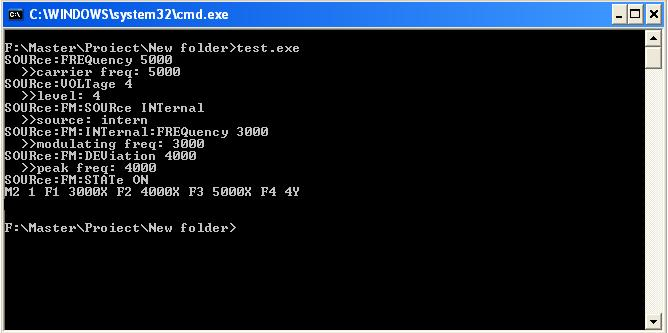
\includegraphics[scale=0.5]{Figuri/cmd_run.JPG}
 \caption{Aplica\c{t}ia rul\^{a}nd \^{i}n modul Internal FM}
 \label{fig_cmd}
\end{figure}

\^{I}n figura \ref{fig_mon} se prezint\u{a} mesajul transmis de program c\u{a}tre portul serial, mesaj capturat cu o aplica\c{t}a de monitorizare a portului serial, Free Serial Port Monitor.
\begin{figure}[htp]
 \centering
 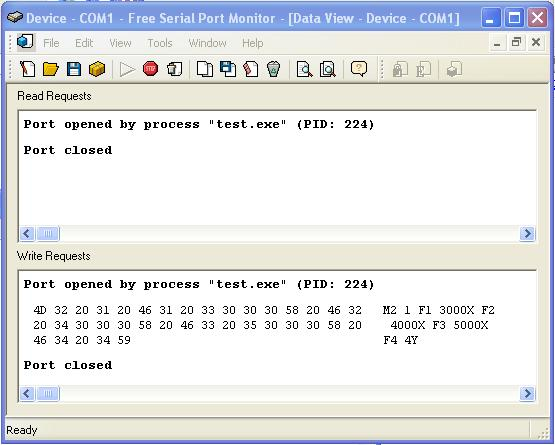
\includegraphics[scale=0.5]{Figuri/com_monitor.JPG}
 \caption{Monitorizarea portului serial}
 \label{fig_mon}
\end{figure}

Figura \ref{figsistem} prezint\u{a} \^{i}ntregul sistem \c{s}i fluxul de date ce are loc.

\begin{figure}[tbp]
  \centering
  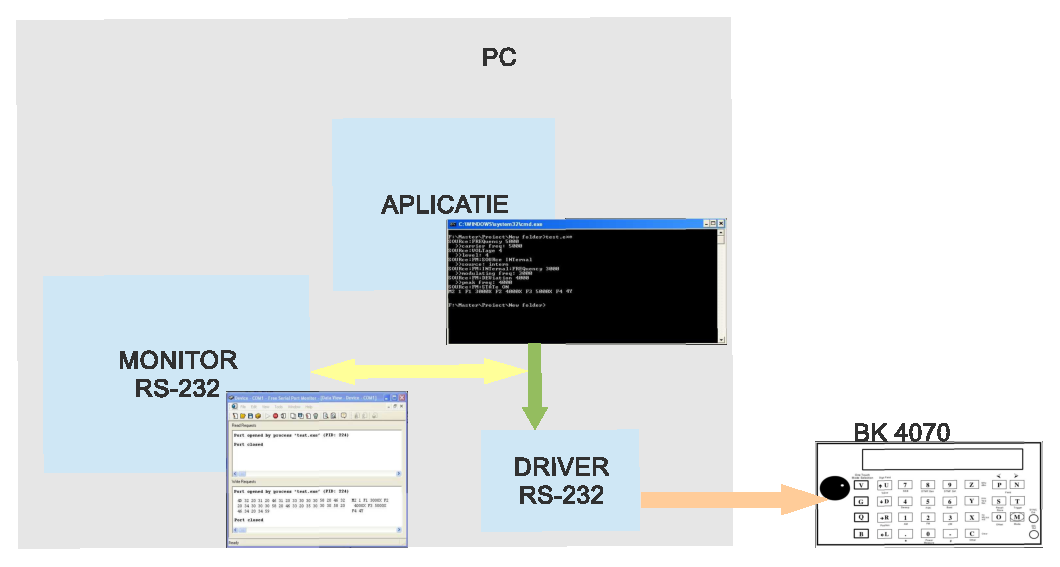
\epsfig{file=Figuri/sistem_.eps,width=1.1\linewidth,clip=}
  \caption{Sistemul implementat}
  \label{figsistem}
\end{figure}
 % Introduction
% Chapter 1

\chapter{Concluzii} % Write in your own chapter title
\label{Capitolul5}
\lhead{Capitolul 5. \emph{Concluzii}} % Write in your own chapter title to set the page header

Implementarea unei interfe\c{t}e SCPI pentru generatorul BK 4070 s-a demonstrat a fi la \^{i}ndem\^{a}n\u{a}, folosind cele doua utilitare Lex \c{s}i Yacc. Interfe\c{t}ei, fiind un rezultat al unui cod C, i se poate extinde oric\^{a}nd func\c{t}ionalitatea, indiferent de platforma pe care se lucreaz\u{a}.

Pentru a se potrivi cu filozofia SCPI, o bun\u{a} implementare ar trebui s\u{a} completeze dinamismul SCPI dar s\u{a}-i men\c{t}in\u{a} \c{s}i coeren\c{t}a. Urm\u{a}toarele caracteristici SCPI au trebuit urm\u{a}rite \^{i}n realizarea acestei interfe\c{t}e:
\begin{itemize}
	\item Extensibilitate - SCPI este proiectat pentru a fi extins, iar versiuni noi vor introduce comenzi noi. O implementare configurabil\u{a} trebuie s\u{a} ofere o modalitate simpl\u{a} de ad\u{a}ugare de noi comenzi;
	\item Portabilitate - o bun\u{a} implementare trebuie s\u{a} fie portabil\u{a};
	\item Reutilizare \c{s}i mentenabilitate - un software bun este reutilizabil. SCPI accept\u{a} fundamental reutilizarea;
	\item Scalabilitate - SCPI defineste unele seturi de comenzi pentru clase similare de instrumente. O bun\u{a} implementare trebuie s\u{a} ia \^{i}n considerare scenarii introduse de diferite instrumente.
\end{itemize}

Aplica\c{t}ia se poate extinde relativ u\c{s}or prin ad\u{a}ugarea urm\u{a}toarelor func\c{t}ionalit\u{a}\c{t}i: folosirea sintaxei prescurtate \c{s}i a comenzilor de interogare a instrumentului.

Un instrument cu suport pentru standardul SCPI va fi \^{i}ntotdeauna preferat datorit\u{a} comenzilor standardizate \c{s}i a sintaxei specifice. Cu ajutorul acestui tip de interfa\c{t}\u{a}, se pot intruduce \^{i}n sistemul de m\u{a}surare \c{s}i control instrumente care au alte avantaje. Av\^{a}nd definit lexicul \^{i}n fi\c{s}ierul Lex, sintaxa se poate modifica cu u\c{s}urin\c{t}\u{a} pentru a satisface comenzile specifice unui alt instrument programabil. 
 % Introduction


%% ----------------------------------------------------------------
% Now begin the Appendices, including them as separate files

\addtocontents{toc}{\vspace{2em}} % Add a gap in the Contents, for aesthetics

\label{Bibliography}
\lhead{\emph{Bibliography}}  % Change the left side page header to "Bibliography"
\bibliographystyle{unsrtnat}  % Use the "unsrtnat" BibTeX style for formatting the Bibliography
\bibliography{Bibliography}  % The references (bibliography) information are stored in the file named "Bibliography.bib"


\appendix % Cue to tell LaTeX that the following 'chapters' are Appendices

% Appendix A

\chapter{Sursa fi\c{s}ierului Lex}
\label{AnexaA}
\lhead{Anexa A. \emph{Sursa fi\c{s}ierului Lex}}

\begin{lstlisting}
%{
#include <stdio.h>
#include <string.h>
#include "y.tab.h"
char fr, sr;
%}

%%
SOURce:VOLTage		return VOLTAGE;

SOURce:AM:SOURce	return AM_SOURCE;
SOURce:AM:DEPTh		return AM_DEPTH;
SOURce:AM:INTernal:FREQuency	return AM_FREQ;
SOURce:APPLy:SIN	return AM_FREQ1;

SOURce:FM:SOURce	return FM_SOURCE;
SOURce:FM:INTernal:FREQuency	return FM_FREQ;
SOURce:FM:DEViation	return FM_PEAK;
SOURce:FREQuency	return FREQ;
SOURce:FM:STATe		return FM_START;

SOURce:SWEep:STATe	return SW_START;
SOURce:FREQuency:STARt	return SW_FR_START;
SOURce:FREQuency:STOP	return SW_FR_STOP;
SOURce:SWEep:SPACing	return SW_LIN_LOG;
SOURce:SWEep:DIRection	return SW_UP_DOWN;
SOURce:SWEep:TIME	return SW_TIME;

SOURce:PM:SOURce	return PM_SOURCE;
SOURce:PM:INTernal:FREQuency	return PM_FREQ;
SOURce:PM:DEViation	return PM_DEVIATION;
SOURce:PM:STATe		return PM_START;

SOURce:FREQuency:FSKey:SOURce	return FSK_SOURCE;
SOURce:FREQuency:FSKey:MARK	return FSK_MARK;
SOURce:FREQuency:FSKey:SPACe	return FSK_SPACE;
SOURce:FSKey:STATe	return FSK_START;

INTernal	{yylval=yytext;return INTERNAL;}
EXTernal	{yylval=yytext;return EXTERNAL;}
SOURce:AM:STATe	return START;
ON	return OK;
LINear	return LINEAR;
LOGarithmic	return LOGARITHMIC;
UP	return SW_UP;
DOWN	return SW_DOWN;
SINusoid	return SINUSOID;
FUNCtion	return FUNCTION;
TRIGger		return TRIGGER;
NOISe		return NOISE;
TRIangle	return TRIANGLE;

[0-9]+			{yylval=atoi(yytext);return NUMBER;}
\n
[ \t]+


%%
\end{lstlisting}
	% Appendix Title

% Appendix A

\chapter{Sursa fi\c{s}ierului Yacc}
\label{AnexaB}
\lhead{Anexa B. \emph{Sursa fi\c{s}ierului Yacc}}

\begin{lstlisting}
%{
#include <stdio.h>
#include <string.h>
#include <stdlib.h>
#include <windows.h>
#include <tchar.h>
HANDLE hPort;
char DataBuffer[];
char* surs;
char* spac;
char* dir;
int freq1,freq,depth,peak,start_freq,stop_freq,time,deviat,level,n1,n2,len;
%}

%token AM_SOURCE AM_DEPTH AM_FREQ AM_FREQ1 INTERNAL EXTERNAL NUMBER START VIRGULA VOLTAGE
%token FM_SOURCE FM_FREQ FM_PEAK FREQ FM_START OK
%token SW_START SW_FR_START SW_FR_STOP SW_LIN_LOG SW_UP_DOWN SW_TIME LINEAR LOGARITHMIC SW_UP SW_DOWN
%token PM_SOURCE PM_FREQ PM_DEVIATION PM_START
%token SINUSOID FUNCTION TRIGGER NOISE TRIANGLE
%token FSK_SOURCE FSK_MARK FSK_SPACE FSK_START
%%

commands: /* empty */
	| commands command
	;
numbers:
	numbers NUMBER	
	|
	NUMBER
	;
command:
	comm numbers
	|
	comm sursa
	|
	comm spacing
	|
	comm direct
	|
	comm
	;
sursa:
	INTERNAL	{surs="1";printf(" intern\n");}
	|
	EXTERNAL	{surs="2";printf(" extern\n");}
	;
spacing:
	LINEAR		{spac="1";printf(" linear\n");}
	|
	LOGARITHMIC	{spac="0";printf(" logarithmic\n");}
	;
direct:
	SW_UP	{dir="0";printf(" up\n");}
	|
	SW_DOWN	{dir="1";printf(" down\n");}
	;
comm:
	AM_FREQ1 {printf("  >>carrier freq:");}
	| VOLTAGE NUMBER {printf("  >>level: %i\n", $2);level=$2;}
	| AM_SOURCE	{printf("  >>source:");}
	| AM_DEPTH NUMBER	{printf("  >>percentage modulation: %i\n",$2);depth=$2;}
	| AM_FREQ NUMBER	{printf("  >>modulating freq: %i\n", $2);freq=$2;}
	| START	OK	{
				if(surs=="1")
					{
						printf("M1 %s F1 %iX F2 %iZ F3 %iX F4 %iY\n", surs, freq, depth, freq1, level);
						sprintf(DataBuffer,"M1 %s F1 %iX F2 %iZ F3 %iX F4 %iY", surs, freq, depth, freq1, level);
						len = strlen(DataBuffer);
						WriteString(DataBuffer, len);
					}
				else
					{
						printf("M1 %s F1 0Z F2 %iX F3 %iY\n", surs, freq1,level);
						sprintf(DataBuffer,"M1 %s F1 0Z F2 %iX F3 %iY", surs, freq1,level);
						len = strlen(DataBuffer);
						WriteString(DataBuffer, len);
					}
			}
	| FM_SOURCE	{printf("  >>source:");}
	| FM_FREQ NUMBER	{printf("  >>modulating freq: %i\n",$2);freq=$2;}
	| FM_PEAK NUMBER	{printf("  >>peak freq: %i\n",$2);peak=$2;}
	| FREQ NUMBER	{printf("  >>carrier freq: %i\n",$2);freq1=$2;}
	| FM_START OK	{
		if(surs=="1")
			{
				printf("M2 %s F1 %iX F2 %iX F3 %iX F4 %iY\n", surs, freq, peak, freq1, level);
				sprintf(DataBuffer,"M2 %s F1 %iX F2 %iX F3 %iX F4 %iY", surs, freq, peak, freq1, level);
				len = strlen(DataBuffer);
				WriteString(DataBuffer, len);
			}
		else
			{
				printf("M2 %s F1 %iX F2 %iX F3 %iY\n", surs, peak, freq1, level);
				sprintf(DataBuffer,"M2 %s F1 %iX F2 %iX F3 %iY", surs, peak, freq1, level);
				len = strlen(DataBuffer);
				WriteString(DataBuffer, len);
			}
	}
	| SW_FR_START NUMBER	{printf("  >>start freq: %i\n", $2);start_freq=$2;}
	| SW_FR_STOP NUMBER	{printf("  >>stop freq: %i\n", $2);stop_freq=$2;}
	| SW_LIN_LOG	{printf("  >>lin\log sweep:");}
	| SW_UP_DOWN	{printf("  >>direction:");}
	| SW_TIME NUMBER	{printf("  >>sweep time: %i\n", $2);time=$2;}
	| SW_START OK	{
				printf("M4 F1 %iX F2 %iX F3 %s F4 %i F5 %s F6 %iX F7 %iY\n", start_freq, stop_freq, spac, surs, dir, time, level);
				sprintf(DataBuffer,"M4 F1 %iX F2 %iX F3 %s F4 %i F5 %s F6 %iX F7 %iY", start_freq, stop_freq, spac, surs, dir, time, level);
				len = strlen(DataBuffer);
				WriteString(DataBuffer, len);
			}
	| PM_SOURCE	{printf("  >>source:");}
	| PM_FREQ NUMBER	{printf("  >>modulating freq: %i\n", $2);freq=$2;}
	| PM_DEVIATION NUMBER	{printf("  >>peak phase deviation: %i\n", $2);deviat=$2;}
	| PM_START OK	{
				if(surs=="1")
				{			
					printf("M3 %s F1 %iX F2 %iX F3 %iX F4 %iY\n", surs, freq, deviat, freq1, level);
					sprintf(DataBuffer,"M3 %s F1 %iX F2 %iX F3 %iX F4 %iY", surs, freq, deviat, freq1, level);
					len = strlen(DataBuffer);
					WriteString(DataBuffer, len);
				}
				else
				{			
					printf("M3 %s F1 %i F2 %iX F3 %iY\n", deviat, freq1, level);
					sprintf(DataBuffer,"M3 %s F1 %i F2 %iX F3 %iY", deviat, freq1, level);
					len = strlen(DataBuffer);
					WriteString(DataBuffer, len);
				}
	}
	| FUNCTION SINUSOID 	{
					printf("B F1 %iX F2 %iY\n", freq1, level);
					sprintf(DataBuffer,"B F1 %iX F2 %iY", freq1, level);
					len = strlen(DataBuffer);
					WriteString(DataBuffer, len);
				}
	| FUNCTION NOISE	{
					printf("V F1 3 F2 %i F3 %iX F4 %iY\n", surs, freq1, level);
					sprintf(DataBuffer, "V F1 3 F2 %i F3 %iX F4 %iY", surs, freq1, level);
					len = strlen(DataBuffer);
					WriteString(DataBuffer, len);
				}
	| FUNCTION TRIANGLE	{
					printf("V F1 2 F2 %i F3 %iX F4 %iY\n", surs, freq, level);
					sprintf(DataBuffer, "V F1 2 F2 %i F3 %iX F4 %iY", surs, freq, level);
					len = strlen(DataBuffer);
					WriteString(DataBuffer, len);
				}
	| TRIGGER {printf("  >>trigger source:");}
	| FSK_MARK NUMBER {printf("  >>mark freq: %i\n", $2);n1=$2;}
	| FSK_SPACE NUMBER {printf("  >>space freq: %i\n", $2);n2=$2;}
	| FSK_SOURCE {printf("  >>source:");}
	| FSK_START OK {
		if(surs=="1")
			{
				printf("M5 %s F1 %iX F2 %iX F3 %iX %iY\n", surs, freq1, n1, n2, level);
				sprintf(DataBuffer,"M5 %s F1 %iX F2 %iX F3 %iX %iY", surs, freq1, n1, n2, level);
				len = strlen(DataBuffer);
				WriteString(DataBuffer, len);
			}
		else
			{
				printf("M5 %s F1 %iX F2 %iX F3 %iY\n", surs,n1,n2,level); 
				sprintf(DataBuffer,"M5 %s F1 %iX F2 %iX F3 %iY", surs,n1,n2,level);
				len = strlen(DataBuffer);
				WriteString(DataBuffer, len);
			}
	}	
	;
%%

//--------------------
HANDLE ConfigureSerialPort(LPCSTR  lpszPortName)
{
    HANDLE hComm = NULL;
    DWORD dwError;
    DCB PortDCB;
    COMMTIMEOUTS CommTimeouts;
    hComm = CreateFile (lpszPortName,
        GENERIC_READ | GENERIC_WRITE,
        0,
        NULL,
        OPEN_EXISTING,
        0,
        NULL);

    PortDCB.DCBlength = sizeof (DCB);
    GetCommState (hComm, &PortDCB);
    PortDCB.BaudRate = 9600;
    PortDCB.fBinary = TRUE;
    PortDCB.fParity = TRUE;
    PortDCB.fOutxCtsFlow = FALSE;
    PortDCB.fOutxDsrFlow = FALSE;
    PortDCB.fDtrControl = DTR_CONTROL_ENABLE;
    PortDCB.fDsrSensitivity = FALSE;
    PortDCB.fTXContinueOnXoff = TRUE;
    PortDCB.fOutX = FALSE;
    PortDCB.fInX = FALSE;
    PortDCB.fErrorChar = FALSE;
    PortDCB.fNull = FALSE;
    PortDCB.fRtsControl = RTS_CONTROL_ENABLE;
    PortDCB.fAbortOnError = FALSE;
    PortDCB.ByteSize = 8;
    PortDCB.Parity = NOPARITY;
    PortDCB.StopBits = ONESTOPBIT;

    if (!SetCommState (hComm, &PortDCB))
    {
        printf("Could not configure serial port\n");
        return NULL;
    }

    GetCommTimeouts (hComm, &CommTimeouts);
    CommTimeouts.ReadIntervalTimeout = MAXDWORD;
    CommTimeouts.ReadTotalTimeoutMultiplier = 0;
    CommTimeouts.ReadTotalTimeoutConstant = 0;
    CommTimeouts.WriteTotalTimeoutMultiplier = 0;
    CommTimeouts.WriteTotalTimeoutConstant = 0;
    if (!SetCommTimeouts (hComm, &CommTimeouts))
    {
        printf("Could not set timeouts\n");
        return NULL;
    }
    return hComm;
}

void ClosePort()
{
    CloseHandle(hPort);
    return;
}

BOOL WriteByte(BYTE bybyte)
{
    DWORD iBytesWritten=0;
    DWORD iBytesToRead = 1;
    if(WriteFile(hPort,(LPCVOID) 
        &bybyte,iBytesToRead,&iBytesWritten,NULL)==0)
        return FALSE;
    else return TRUE;
}

BOOL WriteString(const void *instring, int length)
{
    int index;
    BYTE *inbyte = (BYTE *) instring;
    for(index = 0; index< length; ++index)
    {
        if (WriteByte(inbyte[index]) == FALSE)
            return FALSE;
    }
    return TRUE;
}
//---------------------

int yywrap()
{
	return 1;
}

void prompt()
{
	printf(">");
}

main()
{
	//prompt();
    hPort = ConfigureSerialPort("COM1");
    if(hPort == NULL)
    {
        printf("Com port configuration failed\n");
        return -1;
    }
	yyparse();
	ClosePort();
}

  int yyerror(void)
  {
      printf("Error\n");
      exit(1);
  }


\end{lstlisting}
 % Appendix Title

%\input{./Appendices/AppendixC} % Appendix Title

\addtocontents{toc}{\vspace{2em}}  % Add a gap in the Contents, for aesthetics
\backmatter

%% ----------------------------------------------------------------

\end{document}  % The End
%% ----------------------------------------------------------------